\documentclass[german,oneside,color]{htldipl}
% Zulässige Class Options: 
%   Hauptsprache: german (default), english
%   Doppelseitig: oneside (default), twoside
%   Syntax-Highlighting: color (default), black

% die folgende Zeile einkommentieren für Arial-Ähnliche Schriftart
%\renewcommand{\familydefault}{\sfdefault}

\graphicspath{{images/}}    % Bilderverzeichnis

\usepackage[paper=a4paper,margin=3cm]{geometry}
\usepackage[parfill]{parskip}

\makeindex[title=Index]
\makeindex[name=allgemein, title=Allgemeiner Index]
\makeindex[name=name,title={Autoren Index}]
\makeindex[name=title,columns=1,title={Literatur Index}]
\indexsetup{level=\subsection*, toclevel=subsection, noclearpage}


\makeatletter
\@ifpackageloaded{biblatex_legacy}
  {\DeclareIndexNameFormat{default}{%
     \usebibmacro{index:name}{\index[name]}{#1}{#3}{#5}{#7}}}
  {\DeclareIndexNameFormat{default}{%
     \usebibmacro{index:name}{\index[name]}
       {\namepartfamily}
       {\namepartgiven}
       {\namepartprefix}
       {\namepartsuffix}}}
\makeatother

\DeclareIndexFieldFormat{indextitle}{%
  \usebibmacro{index:title}{\index[title]}{#1}}

\renewbibmacro*{bibindex}{%
  \ifbibindex
    {\indexnames{author}%
     \indexnames{editor}%
     \indexnames{translator}%
     \indexnames{commentator}%
     \indexfield{indextitle}}
    {}}

\makeatletter
\DeclareCiteCommand{\repeatfootcite}[\cbx@wrap]
  {\gdef\cbx@keys{}}
  {\xappto\cbx@keys{\thefield{entrykey},}}
  {}
  {\ifcsundef{cbx@lastin@\cbx@keys @\strfield{postnote}}
     {\csnumgdef{cbx@lastin@\cbx@keys @\strfield{postnote}}{-1}}{}%
   \ifsamepage{\value{instcount}}{\csuse{cbx@lastin@\cbx@keys @\strfield{postnote}}}
     {\footnotemark[\csuse{cbx@lastfn@\cbx@keys @\strfield{postnote}}]}
     {\xappto\cbx@cite{\noexpand\footcite%
        [\thefield{prenote}][\thefield{postnote}]{\cbx@keys}%
        \csnumgdef{cbx@lastfn@\cbx@keys @\strfield{postnote}}{\value{\@mpfn}}%
        \csnumgdef{cbx@lastin@\cbx@keys @\strfield{postnote}}{\value{instcount}}}}}

\newrobustcmd{\cbx@wrap}[1]{#1\cbx@cite\gdef\cbx@cite{}}
\def\cbx@cite{}
\makeatother

\makeglossaries
\loadglsentries{glossary}					%beinhaltet Daten für das Glossar
\addbibresource{literatur.bib}     %beinhaltet Daten für das Literarturverzeichnis

%%%----------------------------------------------------------
\begin{document}
%%%----------------------------------------------------------
%Einstellungen an die eigene Diplomarbeit anpassen
\title{Entwurf eines Versuchstandes für Kreiselpumpen}
\abteilung{Maschineningenieurwesen}
%\schwerpunkt{} wenn kein Ausbildungsschwerpunkt vorhanden ist z.B. Informatik
\schwerpunkt{Ausbildungsschwerpunkt Automatisierungstechnik}
\studienort{Wiener Neustadt}
\schule{HTBLuVA Wiener Neustadt}
\schullogo{htl.jpeg}
\abgabejahr{2010/11}
\betreuerA{Dr.\ Walter Turbo}
\betreuerB{Dipl.-Ing.\ Hans Kreisel}
\betreuerC{Kurt Heidenheim}
\betreuerD{Ing.\ Reiner Tischler}
%\betreuerD{} leer lassen wenn nicht vorhanden
\schuelerA{Maximilian MAIER}
\evidenzA{5AHMIA-17}
\subthemaA{Konstruktion des Versuchstandes}
\schuelerB{Elisabeth MUSTER}
\evidenzB{5AHMIA-19}
\subthemaB{Erstellen der Pumpenkennlinien}
\schuelerC{Peter ZAPFEL}
\evidenzC{5AHMIA-24}
\subthemaC{Integration des Versuchstandes in die bestehende Softwarelösung für die Kennlinien}
\schuelerD{Otto BAUER}
\evidenzD{5BHMIA-02}
\subthemaD{Subthema D}
\schuelerE{Elfriede NURNBERG-ATTACH}
\evidenzE{5BHMIA-20}
\subthemaE{Subthema E}
%\schuelerE{} leer lassen wenn nicht vorhanden
%\evidenzE{}
%\subthemaE{}

%%%----------------------------------------------------------
\frontmatter
\maketitle
\tableofcontents
%%%----------------------------------------------------------

\chapter{Vorwort}

Dies ist \textbf{Version \htldiplDate} der \latex-Dokumentenvorlage für 
die Diplomarbeiten an der HTL Wiener Neustadt, basierend auf der
Vorlage für Abschlussarbeiten an der FH Hagenberg erstellt von Dr.\ Wilhelm
Burger\footnote{\url{http://www.fh-hagenberg.at/staff/burger/diplomarbeit/}}.

Die Verwendung dieser Vorlage ist jedermann freigestellt und an
keinerlei Erwähnung gebunden. Allerdings -- wer sie als Grundlage
seiner eigenen Arbeit verwenden möchte, sollte nicht einfach
("`ung'schaut"') darauf los werken, sondern zumindest die
wichtigsten Teile des Dokuments \emph{lesen} und nach Möglichkeit
auch beherzigen. Die Erfahrung zeigt, dass dies die Qualität der
Ergebnisse deutlich zu steigern vermag.

Der Quelltext zu diesem Dokument sowie das zugehörige
\latex-Paket sind in der jeweils aktuellen Version online
verfügbar unter
%
\begin{quote}
\url{http://unterricht.schermann.org/index.php/Diplomarbeitsvorlage_Latex}
\end{quote}
%
Trotz großer Mühe enthält dieses Dokument zweifellos Fehler und Unzulänglichkeiten
-- Kommentare, Verbesserungsvorschläge und passende Ergänzungen
sind daher stets willkommen, am einfachsten per E-Mail direkt an mich:
\begin{center}%
\begin{tabular}{l}
\nolinkurl{w.schermann@htlwrn.ac.at} \\
Wolfgang Schermann MSc \\
HTL Wiener Neustadt -- Informatik\\
Austria
\end{tabular}
\end{center}

\noindent
Übrigens, hier im Vorwort kann man kurz auf die Entstehung  des Dokuments eingehen.
Hier ist auch der Platz für allfällige Danksagungen (\zB an den Betreuer, 
den Begutachter, die Familie, den Hund, ...), Widmungen und philosophische 
Anmerkungen. Das sollte man allerdings auch nicht übertreiben und sich auf 
einen Umfang von maximal zwei Seiten beschränken.




				%ggfs. weglassen
%Inkludiert die 4. vorgeschriebenen Seiten an Dokumentation aus dem gedruckten PDF-Formular
%Das Formular erst vor der Abgabe vollständig ausfüllen, da z.B. das Bild zur Diplomarbeit vorher nicht vorhanden sein wird
\begingroup
\makeatletter
\newpage
\@twosidefalse
\includepdf[pages=1-1,pagecommand={\chapter[Diplomarbeit Dokumentation]{}}]{pdf/Formular-printed.pdf}
\includepdf[pages=2-2,pagecommand={\thispagestyle{plain}}]{pdf/Formular-printed.pdf}
\includepdf[pages=3-3,pagecommand={\chapter[Diploma Thesis Documentation]{}}]{pdf/Formular-printed.pdf}
\includepdf[pages=4-4,pagecommand={\thispagestyle{plain}}]{pdf/Formular-printed.pdf}
\endgroup
\chapter{Kurzfassung}

An dieser Stelle steht eine Zusammenfassung der Arbeit, Umfang
max.\ 1 Seite. Im Unterschied zu anderen Kapiteln ist die
Kurzfassung (und das Abstract) üblicherweise nicht in Abschnitte
und Unterabschnitte gegliedert. 
Auch Fußnoten sind hier falsch am Platz.

Kurzfassungen werden übrigens häufig -- zusammen mit Autor und Titel
der Arbeit -- %
in Literaturdatenbanken aufgenommen. Es ist daher darauf zu
achten, dass die Information in der Kurzfassung für sich 
\emph{allein} (\dah ohne weitere Teile der Arbeit) zusammenhängend und
abgeschlossen ist. Insbesondere werden an dieser Stelle (wie \ua
auch im \emph{Titel} der Arbeit und im \emph{Abstract})
normalerweise \emph{keine Literaturverweise} verwendet! Falls man
unbedingt solche benötigt -- etwa weil die Arbeit eine
Weiterentwicklung einer bestimmten, früheren Arbeit darstellt --,
dann sind \emph{vollständige} Quellenangaben in der Kurzfassung
selbst notwendig, \zB %
[\textsc{Zobel} J.: \textit{Writing for Computer Science -- The Art of
Effective Commu\-nica\-tion}. Springer-Verlag, Singa\-pur, 1997].

Weiters sollte man daran denken, dass bei der Aufnahme in Datenbanken
Sonderzeichen oder etwa Aufzählungen mit "`Knödellisten"' in der
Regel verloren gehen. Dasselbe gilt natürlich auch für das 
\emph{Abstract}.


Inhaltlich sollte die Kurzfassung \emph{keine} Auflistung der
einzelnen Kapitel sein (dafür ist das Einleitungskapitel
vorgesehen), sondern dem Leser einen kompakten, inhaltlichen
Überblick über die gesamte Arbeit verschaffen. Der hier verwendete
Aufbau ist daher zwangsläufig anders als der in der Einleitung.
		
\chapter{Abstract}

\begin{english} %switch to English language rules
This should be a 1-page (maximum) summary of your work in English.
%und hier geht dann das Abstract weiter...
\end{english}

Im englischen Abstract sollte inhaltlich das Gleiche
stehen wie in der deutschen Kurzfassung. Versuchen Sie daher, die
Kurzfassung prä\-zise umzusetzen, ohne aber dabei Wort für Wort zu
übersetzen. Beachten Sie bei der Übersetzung, dass gewisse
Redewendungen aus dem Deutschen im Englischen kein Pendant haben
oder völlig anders formuliert werden müssen und dass die
Satzstellung im Englischen sich (bekanntlich) vom Deutschen stark
unterscheidet (mehr dazu in Abschn.\ \ref{sec:englisch}). Es
empfiehlt sich übrigens -- auch bei höchstem Vertrauen in die
persönlichen Englischkenntnisse -- eine kundige Person für das
"`proof reading"' zu engagieren.

Die richtige Übersetzung für "`Diplomarbeit"' ist übrigens
schlicht \emph{thesis}, allenfalls  "`diploma thesis"', auf keinen Fall aber "`diploma work"' oder gar "`dissertation"'. 

Übrigens sollte für diesen Abschnitt die \emph{Spracheinstellung} in \latex\ von Deutsch
auf Englisch umgeschaltet werden, um die richtige Form der
Silbentrennung zu erhalten, die richtigen Anführungszeichen muss
man allerdings selbst setzen %
(s.\ dazu Abschnitt \ref{sec:sprachumschaltung} %
bzw.\ \ref{sec:anfuehrungszeichen}).
			

%%%----------------------------------------------------------
\mainmatter           %Hauptteil (ab hier arab. Seitenzahlen)
%%%----------------------------------------------------------

\chapter{Einleitung}
\label{cha:Einleitung}

\section{Zielsetzung}
Dieses Dokument ist als vorwiegend technische Starthilfe für das
Erstellen einer Diplomarbeit mit \latex
gedacht und ist die Weiterentwicklung einer früheren
Vorlage\footnote{Nicht mehr verfügbar.} für das Arbeiten mit
Microsoft \emph{Word}. Während ursprünglich daran gedacht war, die
bestehende Vorlage einfach in \latex zu übernehmen, wurde rasch
klar, dass allein aufgrund der großen Unterschiede zum Arbeiten
mit \emph{Word} ein gänzlich anderer Ansatz notwendig wurde. Dazu
kamen zahlreiche Erfahrungen mit Diplomarbeiten in den
nachfolgenden Jahren, die zu einigen zusätzlichen Hinweisen Anlass gaben.

Das vorliegende Dokument dient einem zweifachen Zweck: 
\emph{erstens} als Erläuterung und Anleitung, \emph{zweitens} als
direkter Ausgangspunkt für die eigene Arbeit. Angenommen wird,
dass der Leser bereits über elementare Kenntnisse im Umgang mit
\latex verfügt. In diesem Fall sollte -- eine einwandfreie
Installation der Software vorausgesetzt -- der Arbeit nichts mehr
im Wege stehen. Auch sonst ist der Start mit \latex\ nicht
schwierig, da viele hilfreiche Informationen auf den zugehörigen
Webseiten zu finden sind (s.\ Abschn.~\ref{sec:latex}).





\section{Warum {\latex}?}

Diplomarbeiten, Dissertationen und Bücher im
technisch-natur\-wissen\-schaft\-lichen Bereich werden
traditionell mithilfe des Textverarbeitungssystems \latex
\cite{Lamport94,Lamport95} gesetzt. Das hat gute Gründe, denn
\latex ist bzgl.\ der Qualität des Druckbilds, des Umgangs mit
mathematischen Elementen, Literaturverzeichnissen etc.\
unübertroffen und ist noch dazu frei verfügbar. Wer mit \latex
bereits vertraut ist, sollte es auch für die Diplomarbeit
unbedingt in Betracht ziehen, aber auch für den Anfänger sollte
sich die zusätzliche Mühe am Ende durchaus lohnen.

Für den professionellen elektronischen Buchsatz wurde bisher
häufig \emph{Adobe Framemaker} verwendet, allerdings ist diese
Software teuer und komplex. Eine modernere Alternative dazu ist
\emph{Adobe InDesign}, wobei allerdings die Erstellung
mathematischer Elemente und die Verwaltung von Literaturverweisen
zur Zeit nur rudimentär unterstützt werden.%
\footnote{Angeblich werden aber für den (sehr sauberen) Schriftsatz 
in \emph{InDesign} ähnliche Algorithmen wie in \latex\ verwendet.}

Microsoft \emph{Word} gilt im Unterschied zu \latex, 
\emph{Framemaker} und \emph{InDesign} übrigens nicht als professionelle
Textverarbeitungssoftware, obwohl es immer häufiger auch von
großen Verlagen verwendet wird.%
\footnote{Siehe auch \url{http://latex.tugraz.at/mythen.php}.}
Das Schriftbild in \emph{Word}
lässt -- zumindest für das geschulte Auge -- einiges zu wünschen
übrig und das Erstellen von Büchern und ähnlich großen Dokumenten
wird nur unzureichend unterstützt. Allerdings ist \emph{Word} sehr
verbreitet, flexibel und vielen Benutzern zumindest oberflächlich
vertraut, sodass das Erlernen eines speziellen Werkzeugs wie
\latex\ ausschließlich für das Erstellen einer Diplomarbeit
manchen verständlicherweise zu mühevoll ist. Man sollte es daher
niemandem übel nehmen, wenn er/sie sich auch bei der Diplomarbeit
auf \emph{Word} verlässt. Im Endeffekt lässt sich mit etwas
Sorgfalt (und ein paar Tricks) auch damit ein durchaus akzeptables
Ergebnis erzielen. Für alle, die so denken, finden sich in
Kap.~\ref{chap:Word} einige spezielle Hinweise zum Arbeiten mit
\emph{Word}. Ansonsten sollten für \emph{Word}-Benutzer aber auch
andere Teile dieses Dokuments von Interesse sein, insbesondere die
Abschnitte über Abbildungen und Tabellen
(Kap.~\ref{chap:Abbildungen}) und mathematische Elemente
(Kap.~\ref{chap:Mathematik}).






Übrigens, genau hier am Ende des Einleitungskapitels (und nicht
etwa in der Kurzfassung) ist der richtige Platz, um die
inhaltliche Gliederung der nachfolgenden Arbeit zu beschreiben.
Hier soll dargestellt werden, welche Teile (Kapitel) der Arbeit
welche Funktion haben und wie sie inhaltlich zusammenhängen. Auch
die Inhalte des \emph{Anhangs} -- sofern vorgesehen -- sollten hier
kurz beschrieben werden.


\chapter{Die Diplomschrift}
\label{cha:Diplomschrift}



\section{Elemente der Diplomschrift}

Jede Diplomschrift ist anders und dennoch sind sich gute
Arbeiten in ihrer Struktur meist sehr ähnlich, \va\ bei
technischen Themen. Als Startpunkt bewährt hat sich die folgende
simple Grundstruktur, die man natürlich vari\-ieren und beliebig
verfeinern kann:
%
\begin{enumerate}
\item \textbf{Einführung und Motivation}: Was ist die Problem- oder Aufgabenstellung und
warum sollte man sich dafür interessieren?
\item \textbf{Präzisierung des Themas}: Hier beschreibt man den aktuellen Stand der Technik
oder Wissenschaft ("`State-Of-The-Art"'), zeigt bestehende
Defizite oder offene Fragen auf und entwickelt daraus die
Stoßrichtung der eigenen Arbeit.
\item \textbf{Eigener Ansatz}: Das ist natürlich der Kern der Arbeit. Hier
wird gezeigt, wie man die vorher beschriebene Aufgabenstellung löst und --
häufig in Form eines Programms%
\footnote{\emph{Prototyp} ist in diesem Zusammenhang ein gerne benutzter Begriff, der im Deutschen
allerdings oft unrichtig dekliniert wird. Richtig ist: der \emph{Prototyp}, des \emph{Prototyps}, dem/den \emph{Protototyp} -- falsch hingegen \zB: des \emph{Prototyp\underline{en}}!
} --
realisiert, ergänzt durch illustrative Beispiele.
\item \textbf{Zusammenfassung}: Was wurde erreicht und welche Ziele sind
noch offen geblieben, wo könnte man weiter arbeiten?
\end{enumerate}
%
Natürlich ist auch ein gewisser dramaturgischer Aufbau der Arbeit
wichtig, wobei man bedenken muss, dass der Leser in der Regel nur
wenig Zeit hat und -- anders als etwa bei einem Roman -- seine
Geduld nicht auf die lange Folter gespannt werden darf. Erklären
Sie bereits in der Einführung (und nicht erst im letzten Kapitel),
wie Sie an die Sache herangehen, welche Lösungen Sie vorschlagen
und wie erfolgreich Sie damit waren.

Übrigens, auch Fehler und Sackgassen darf (und sollte) man
beschreiben, ihre Kenntnis hilft oft doppelte Experimente und
weitere Fehler zu vermeiden und ist damit sicher nützlicher als
jede Schönfärberei.


\section{Diplomschriften in Englisch}
\label{sec:englisch}

Diese Vorlage ist zunächst darauf abgestellt, dass die
Diplomschrift in deutscher Sprache erstellt wird. Vor allem bei
Diplomarbeiten, die in Zusammenarbeit mit größeren Firmen oder
internationalen Instituten entstehen, ist es häufig erwünscht,
dass die Diplomschrift zur besseren Nutzbarkeit in englischer
Sprache verfasst wird, und viele Schulen lassen dies in
der Regel auch zu.

Beachten sollte man allerdings, dass das Schreiben dadurch nicht
einfacher wird, auch wenn einem Worte und Sätze im Englischen
scheinbar leichter "`aus der Feder"' fließen. Gerade im Bereich
der Informatik erscheint durch die Dominanz englischer
Fachausdrücke das Schreiben im Deutschen mühsam und das Ausweichen
ins Englische daher besonders attraktiv. Das ist jedoch
trügerisch, da man die eigene Fertigkeit in der Fremdsprache
(trotz der meist langjährigen Schulbildung) häufig überschätzt.
Prägnanz und Klarheit gehen leicht verloren und bisweilen ist das
Resultat ein peinliches Gefasel ohne Zusammenhang und soliden
Inhalt. Sofern man das Englische nicht wirklich gut beherrscht, ist
es ratsam, zumindest die wichtigsten Teile der Arbeit zunächst in
Deutsch zu verfassen und erst nachträglich zu übersetzen.
Besonders vorsichtig sollte man bei der Übersetzung von scheinbar
vertrauten Fachausdrücken sein. Zusätzlich ist es immer zu
empfehlen, die fertige Arbeit von einem "`native speaker"'
korrigieren zu lassen.



Technisch ist, außer der Spracheinstellung und den
unterschiedlichen Anführungszeichen (s.\
Abschn.~\ref{sec:anfuehrungszeichen}), für eine englische Arbeit
nicht viel zu ändern, allerdings sollte man folgendes beachten:
%
\begin{itemize}
\item  Die Titelseite (mit der Bezeichnung "`Diplomarbeit"') 
ist für die einzureichenden Exemplare jedenfalls in \emph{deutsch} zu halten,
auch wenn der Titel englisch ist. 
\item Ebenso muss neben dem
englischen \emph{Abstract} auch eine deutsche \emph{Kurzfassung}
enthalten sein. %
\item Akademische Titel von Personen haben im Englischen offenbar
weniger Bedeutung als im Deutschen und werden daher meist
weggelassen.
\end{itemize}

\chapter{Zum Arbeiten mit \latex}
\label{cha:ArbeitenMitLatex}



\section{Start}
\label{sec:latex}



\latex ist eine in den Naturwissenschaften sehr verbreitete
und mittlerweile klassische Textverarbeitungssoftware für das Erstellen
großer und komplizierter Dokumente mit professionellem Anspruch.
Das Arbeiten mit \latex erscheint -- zumindest für den ungeübten Benutzer -- %
zunächst schwieriger als mit herkömmlichen Werkzeugen für die
Textverarbeitung.

Zum Ersten ist -- im Unterschied zu den meisten gängigen
Text\-ver\-arbei\-tungs\-prog\-ram\-men -- \latex nicht \textsc{Wysiwyg}%
\footnote{"`What You See Is What You Get."' Es gibt auch 
\textsc{Wysiwyg}-Implementierungen für \latex, 
\zB\ \emph{Scientific WorkPlace} (\url{http://www.mackichan.com}) oder
\emph{LyX} (\url{http://www.lyx.org}), 
die aber teuer \bzw\ relativ langsam sind.},
sondern es handelt sich um eine \emph{Markup Lang\-uage} (wie HTML) -- noch dazu
eine recht komplizierte -- und zugehörige Werkzeuge.
Ungewohnt erscheinen sicher auch die vermeintlich starken
Einschränkungen von \latex,
insbesondere in Bezug auf die Wahl der Schriften und das
Layout. Während man anfangs meint, dass diese Rigidität
die eigene Kreativität beschränkt, bemerkt man mit der Zeit, dass es gerade
dadurch gelingt, sich stärker auf die Inhalte der Arbeit zu
konzentrieren als auf deren äußere Form. Dass am Ende die Form dennoch stimmt,
ist allerdings nur dann gewährleistet, wenn man sich bei den eigenen Modifikationen
der Formate und Parameter äußerste Zurückhaltung auferlegt, es sei denn,
man ist in der Zwischenzeit bereits selbst zum \latex-\emph{Guru} avanciert.

Insgesamt lohnt sich der Aufwand, wie viele meinen, zumal die Diplomarbeit
in jedem Fall (mit oder ohne \latex) ein substantielles Stück Arbeit ist.
Es sollte mithilfe von \latex ein professionell aussehendes
Ergebnis einfacher zu erreichen sein und man wird sich wohl auch einigen
Ärger mit Bugs und Unzulänglichkeiten gängiger Software ersparen.
Zudem könnte es durchaus sein, dass man nebenbei auch sein Auge für
die Feinheiten des Buchsatzes (weiter-) entwickelt.

\subsection{Software}

Zum Arbeiten mit \latex benötigt man -- neben einem Computer -- natürlich Software. Musste man sich früher oft die einzelnen Komponenten von \latex mühevoll zusammensuchen und für die eigene Umgebung konfigurieren, gibt es mittlerweile für die wichtigsten Plattformen (Windows, Mac~Os, Linux) fertige \latex-Installationen, die ohne weiteres Zutun laufen. Die aktuelle Version von \latex\ ist \LaTeXe\ (sprich "`LaTeX zwei e"'). 
Zum Arbeiten mit \latex\ benötigt man zwei Dinge:
%
\begin{itemize}
\item \latex-Installation (Distribution)
\item Texteditor oder Autorenumgebung (Frontend)
%\item PostScript/PDF-Software 
\end{itemize}
%
Sämtliche Komponenten sind kostenlos und für alle gängigen Plattformen verfügbar.


\subsubsection{Windows}

Unter \emph{Windows} (XP, Vista, W7) hat sich folgendes Setup bewährt,
mit dem \ua auch dieses Dokument erstellt wurde:
%
\begin{itemize}
\item \textbf{\latex-Distribution}: \emph{MikTeX 2.8} oder höher.
MikTeX enthält auch alle notwendigen Hilfsprogramme, wie beispielsweise {\tt bibtex}.%
\footnote{\url{http://www.miktex.org}}

%\item \textbf{PDF-Viewer}: \emph{SumatraPDF}%
%\footnote{\url{http://blog.kowalczyk.info/software/sumatrapdf/}}

\item \textbf{Frontend}: \emph{TeXnicCenter}.%
\footnote{\url{http://www.texniccenter.org}}
Grundsätzlich kann man jeden Text-Editor%
\footnote{Unter Windows \zB\ \emph{Ultra\-Edit} (\url{http://www.ultraedit.com})
oder \emph{WinEdit} (\url{http://www.winedit.com}).} verwenden, praktischer ist jedoch eine integrierte \latex-Umgebung wie TeXnicCenter, die einen auch bei 
der Dateiverwaltung, der Verarbeitung der Dokumente und der Fehlerbehandlung unterstützt. Für diese Vorlage wird mindestens die Version 2.0 benötigt, da sonst keine Unicode Unterstützung gegeben ist.\footnote{\url{http://www.texniccenter.org}}
%
\end{itemize}
Beim erstem Mal sollten \emph{MikTeX} und \emph{TeXnicCenter} in genau dieser Reihenfolge installiert werden.

MikTeX sollte so eingerichtet werden, dass fehlende Packete automatisch geladen werden. Beim ersten Erstellen werden dann alle notwendigen Packete aus dem Internet geladen und stehen ab dann lokal zur Verfügung. Das erste Erstellen dauert dadurch allerdings mitunter sehr lange. Sollten trotzdem noch fehlende Packete wie \zB\ \emph{tracklang.sty} angezeigt werden, so muss noch MikTeX aktualiert werden. Update (Admin) im Startmenü von MikTeX unter Maintenance. Das Programm wählt automatisch die richtigen Packete zur Aktualisierung aus.

\subsubsection{Mac~OS}

Unter Mac~OS wurde die aktuelle Vorlage noch nicht getestet. Der folgende Text bezieht sich auf die alte Vorlage und ist möglicherweise nicht mehr korrekt.

Bewährte und weit verbreitete Frontends für den Mac sind \emph{MacTeX}%
\footnote{\url{http://www.tug.org/mactex} -- enthält eine komplette und fertig
konfigurierte LaTeX-Installation für Mac~OS (ca.\ 1.15 GB download).}
und \emph{TeXShop},%
\footnote{\url{http://www.uoregon.edu/~koch/texshop/}}
das üblicherweise zusammen mit der TeX-Distribution \emph{TeX Live} verwendet wird. 
Weit verbreitet ist auch der \emph{TeXworks} Editor, der ebenfalls im MacTeX Package enthalten ist und auch MiKTeX unter Windows beigefügt ist.


\subsubsection{Linux}

Auch unter Linux ist \emph{TeX Live} (\so) eine häufig verwendete TeX-Distri\-bution. 
Als Frontend sind beispielsweise
\emph{Lyx}\footnote{\url{http://www.lyx.org}},
\emph{Kile}\footnote{\url{http://kile.sourceforge.net}} und
\emph{Texmaker}\footnote{\url{http://www.xm1math.net/texmaker}} 
verbreitet.
In manchen gängigen Linux-Versionen ist bereits eine komplette \latex-Distribution enthalten, sodass im besten Fall überhaupt keine zusätzliche Installation notwendig ist.  

Eine interessante Alternative ist die Verwendung von
\emph{Eclipse}\footnote{\url{http://www.eclipse.org}} als plattformunabhängiges Frontend 
(mit dem \emph{TeXlipse}\footnote{\url{http://texlipse.sourceforge.net}}
Plugin).


Zum Nachinstallieren zusätzlicher \latex-Pakete die nicht in der
Standardinstallation enthalten sind gibt es für Linux ebenfalls den MikTeX
Package Manager\footnote{\url{http://wiki.ubuntuusers.de/MiKTeX_Package_Manager}}. Allerdings empfiehlt es sich meist die notwendigen Packete statt dessen über die Softwareverwaltung der Linux-Distribution zu installieren. So kann \zB\ in Ubuntu das Packet \emph{texlive-lang-german} installiert werden um die für diese Vorlage notwendige Unterstützung der deutschen Sprache nachzuinstallieren.

\subsubsection{Automatische Generierung von \latex-Code}
Bei der Erstellung von komplizierterem \latex-Code kann man sich zum Glück
einiger Hilfsmittel bedienen.

\begin{itemize}
\item \emph{Online Latex Equation
Editor}\footnote{\url{http://www.codecogs.com/latex/eqneditor.php}} ist ein
einfach zu bedienender Online Editor für mathematische Formeln.
\item \emph{Writer2\latex}\footnote{\url{http://www.ooowiki.de/Writer2LaTeX}}
ist ein Export-Filter für OpenOffice-Writer mit dem jede Form von Textdokumenten in
\latex-Code umgewandelt werden kann.
\item \emph{Calc2\latex}\footnote{\url{http://www.ooowiki.de/Calc2LaTeX}} ist
ein Export-Makro für OpenOffice-Calc mit dem Tabellen für das Einfügen in \latex
erzeugt werden können.
\item \emph{Dot2Tex}\footnote{\url{http://www.fauskes.net/code/dot2tex}} ist
eine Verbindung von Graphviz nach \latex. Graphen können in \latex eingebunden werden
und die Beschriftungen mit \latex geschrieben werden.
\item \emph{gnuplot}\footnote{\url{http://www.gnuplot.info}} ist ein Programm
zur Erstellen von Diagrammen. Über das \latex-Package gnuplottex kann es direkt in
den \latex-Code integriert werden.
\end{itemize}


\subsection{Literatur}
\label{sec:literatur}

Es ist müßig, ohne geeignete Literatur mit \latex zu beginnen, selbst
als fortgeschrittener Benutzer wird man immer wieder auf Hilfe angewiesen
sein. Erfreulicherweise ist sehr viel Nützliches auch online verfügbar.
Gute Startpunkte sind \zB
%
\begin{itemize}
\item \emph{{\rm\LaTeXe}-Kurzbeschreibung} von Schmidt et al.\ \cite{Schmidt01}
\item \emph{The Not So Short Introduction to {\rm \LaTeXe}}
            von Oetiker et al.\ \cite{Oetiker01}
\end{itemize}
%
\noindent
Als mittlerweile bereits klassisches Handbuch zu \latex ist
%
\begin{itemize}
  \item \emph{A Guide to {\rm\LaTeXe}} von H.~Kopka und P.~Daly \cite{Kopka98}
\end{itemize}
%
zu empfehlen, zu dem es für Interessierte auch zwei vertiefende
Zusatzbände in Deutsch gibt. Zahlreiche weitere Dokumente zu
\latex und verwandten Themen finden sich \ua im Rahmen des {\em
Comprehensive TeX Archive Network} (CTAN) auf
\begin{quote}
	\url{http://www.ctan.org}%
	\footnote{\url{http://www.ctan.org/tex-archive/help/Catalogue/bytopic.html}}\newline
	\url{http://dante.ctan.org}%
	\footnote{\url{http://dante.ctan.org/tex-archive/help/Catalogue/bytopic.html}}\newline
	\url{http://www.tex.ac.uk}
\end{quote}
%
Besonders nützlich sind auch die
\emph{Comprehensive List of {\rm \latex} Symbols} \cite{Pakin01}
und die Beschreibungen wichtiger \latex-Pakete, wie
%
\begin{quote}
	\texttt{babel} \cite{Braams2008},\newline
% \texttt{german}, \texttt{ngerman} \cite{Raichle98},\newline
  \texttt{grahics}, \texttt{graphicx} \cite{Carlisle99},\newline
  \texttt{fancyhdr} \cite{Oostrum97},\newline
  \texttt{caption} \cite{Sommerfeldt07},\newline
  \texttt{subfigure} \cite{Cochran95}.
\end{quote}





\section{Schrift}

\subsection{Schriftarten}

\latex verwendet normalerweise die Schriften der \emph{Computer
Modern}
(CM) Serie, die so wie die \emph{TeX}-Software selbst von Donald Knuth%
\footnote{\url{http://www-cs-staff.stanford.edu/~knuth/}} entwickelt
wurden. Die drei Basis-Schrifttypen der CM-Serie in \latex sind
%
\begin{quote}
\begin{tabular}{lcl}
\textrm{Roman}      & & \verb!\textrm{Roman}!\\
\textsf{Sans Serif} & & \verb!\textsf{Sans Serif}!\\
\texttt{Typewriter} & & \verb!\texttt{Typewriter}!\\
\end{tabular}
\end{quote}
%
\noindent In den Augen vieler Benutzer ist allein die Qualität und
Zeitlosigkeit dieser Schriften ein Grund, \latex für seriöse
Zwecke zu verwenden. Ein weiterer Vorteil der \emph{TeX}-Schriften
ist, dass die unterschiedlichen Schriftfamilien und Schnitte
bezüglich der Größe sehr gut aufeinander abgestimmt sind, was %
beim Arbeiten mit verschiedenen \emph{TrueType}-Schriften (\zB\ in
\emph{Word}) durchaus zum Problem werden kann (\sa\ Kap.\
\ref{chap:Word}).

Darüber hinaus können aber in \latex auch beliebige 
\emph{PostScript}-Schrif\-ten (Type 1) verwendet werden, was allerdings in
der Praxis einiges an "`Tuning"'-Arbeit verlangt. Häufig verwendet
werden \zB\ \emph{Times} und \emph{Palatino}, derzeit ist aber ein Trend 
zurück zu den klassischen CM-Schriften zu beobachten.



\subsection{Texte hervorheben}

Texte können auf unterschiedliche Weise aus dem Fließtext hervorgehoben werden.
\begin{itemize}
%
\item Die Auszeichnung in \textit{Kursivschrift} oder "`italic"' (\verb!\textit{..}!) ist \va\ zum Hervorheben von
Betonungen und Zitaten geeignet, aber auch für
Produktbezeichnungen, Fremdwörter und Variablen im Text, \zB
%
\begin{quote}
\verb!\textit{Variable}! $\rightarrow$ \textit{Variable}
\end{quote}
%
\item {\sl Slanted} %
(\verb!\textsl{..}!) bedeutet eine geneigte Schrift und
unterscheidet sich damit deutlich von \textit{Italic}. Wird
beispielsweise verwendet für die laufenden Kopfzeilen,
Produktbezeichnungen und Markennamen -- zum Vergleich:
%
\begin{quote}
\verb!\textrm{Daimler-Chrysler}! $\rightarrow$ \textrm{Daimler-Chrysler} \newline%
\verb!\textsl{Daimler-Chrysler}! $\rightarrow$ \textsl{Daimler-Chrysler} \newline%
\verb!\textit{Daimler-Chrysler}! $\rightarrow$ \textit{Daimler-Chrysler}
\end{quote}
%
\item \textbf{Boldface} (\verb!\textbf{..}!) wird \ia\ verwendet für 
\textbf{Überschriften}, Bezeichnungen von \textbf{Abbildungen} und 
\textbf{Tabellen}, im Fließtext aber selten:
%
\begin{quote}
\verb!\textbf{Überschriften}! $\rightarrow$ \textbf{Überschriften}
\end{quote}
%
\item \emph{Emphasize} (\verb!\emph!) %
ist normalerweise gleichbedeutend mit \verb!\textit!, wobei
\verb!\emph{..}! allerdings auch bei geschachtelten
Hervorhebungen und im Bereich anderer Schriftschnitte das
"`Richtige"' tut: 
%
\begin{quote}
\setlength{\tabcolsep}{0pt}%
\begin{tabular}{lcl}
\verb!\textrm{Du \emph{auch} hier?}! & $\;\rightarrow\;$ &
    \textrm{Du \emph{auch} hier?}
\\
\verb!\textit{Du \emph{auch} hier?}! & $\;\rightarrow\;$ &
    \textit{Du \emph{auch} hier?} 
\\
\verb!\textsl{Du \emph{auch} hier?}! & $\;\rightarrow\;$ & 
    \textsl{Du \emph{auch} hier?}
\\
\verb!\textbf{Du \emph{auch} hier?}! & $\;\rightarrow\;$ & 
    \textbf{Du \emph{auch} hier?}
\\
\verb!\texttt{Du \emph{auch} hier?}! & $\;\rightarrow\;$ & 
    \texttt{Du \emph{auch} hier?}
\end{tabular}
\end{quote}
%
\item \underline{Unterstreichungen} sind ein Relikt aus der 
Schreibmaschinenära und im modernen Schriftsatz
eigentlich \underline{überflüssig}. Sie sollten daher nur in
Ausnahmefällen verwendet werden, \zB
%
\begin{quote}
\verb!\underline{überflüssig}!%
\footnote{Unterstrichene Texte werden zudem nicht automatisch abgeteilt.}
\end{quote}
%
\end{itemize}



\section{Textstruktur}

\subsection{Absatztrennung}

Absätze werden in {\latex}-Quelltext ausschließlich durch das
Einfügen einer oder mehrerer \textbf{Leerzeilen} voneinander
getrennt, es sind also \emph{keinerlei sonstige Steueranweisungen}
notwendig!
%
\begin{center}
\setlength{\fboxrule}{0.2mm}
\setlength{\fboxsep}{2mm}
\fbox{%
\begin{minipage}{0.9\textwidth}
Besonders die Verwendung von \texttt{\textbackslash\textbackslash} und 
 \texttt{\textbackslash{newline}}
Anweisungen zur Absatztrennung ist ein häufig zu beobachtender \textbf{Fehler}. 
Vor normalen Absätzen auch \emph{nichts} verloren hat die
Anweisung \texttt{\textbackslash{paragraph}\{\}}
-- sie ist in \latex\ (im Unterschied zu HTML)
eine Markierung für Überschriften mit Titel (\su)!
\end{minipage}}
\end{center}

Üblicherweise wird durch {\latex} zwischen aufeinanderfolgenden Ab\-sätzen
\emph{kein} zusätzlicher vertikaler Abstand eingefügt. \footnote{Das ist die
Standardeinstellung in {\latex} und natürlich abhängig von der verwendeten Dokumentenklasse, Style
etc.} 
Allerdings wird die
\emph{erste} Zeile jedes Absatzes (mit Ausnahme des ersten Absatzes
eines Abschnitts) eingerückt, um so die Absatzgrenzen deutlich zu
machen. Dieses Schema hat sich nicht nur im traditionellen
Buchsatz bewährt%
\footnote{Wer es nicht glaubt, sollte sein Bücherregal (oder notfalls das seiner Eltern) nach Gegenbeispielen durchsuchen.}
und sollte auch beibehalten werden, es sei denn
man hat wirklich \emph{sehr} gute Gründe dagegen.
Für alle übrigen Gliederungen im vertikalen Textfluss sind Überschriften (s.\ unten) vorgesehen.

\SuperPar 
Manchmal besteht allerdings der Wunsch, etwa zur Verdeutlichung eines inhaltlichen Sprungs \emph{zwischen} zwei Absätzen einen zusätzlichen Abstand einzufügen, ohne dabei eine neue Überschrift zu setzen. Das kann man gegebenenfalls (wie vor dem aktuellen Absatz passiert) durch 
%
\begin{quote}
\texttt{{\bs}SuperPar} \emph{Manchmal besteht allerdings der Wunsch, \ldots}
\end{quote}
%
erreichen, sollte jedoch sehr sparsam und wirklich \textbf{nur in begründbaren Einzelfällen} verwendet werden.%
\footnote{Das Makro \texttt{{\bs}SuperPar} ist in \texttt{htl.sty} definiert.}




\subsection{Überschriften}
\label{sec:ueberschriften}

\latex\ bietet -- abhängig von der verwendeten Dokumentenklasse --
einen Satz vordefinierter Überschriftformate in folgender Ordnung:
%
\begin{quote}
\verb!\part{!\texttt{\em Titel}\verb!}!%
\footnote{\texttt{part} ist für die Gliederung eines
größeren Werks in mehrere Teile vorgesehen und wird üblicherweise
bei einer Diplomarbeit (und auch in diesem Dokument) nicht
verwendet.}
\newline%
\verb!\chapter{!\texttt{\em Titel}\verb!}! \newline%
\verb!\section{!\texttt{\em Titel}\verb!}! \newline%
\verb!\subsection{!\texttt{\em Titel}\verb!}! \newline%
\verb!\subsubsection{!\texttt{\em Titel}\verb!}! \newline%
\verb!\paragraph{!\texttt{\em Titel}\verb!}! \newline%
\verb!\subparagraph{!\texttt{\em Titel}\verb!}!
\end{quote}
%

\paragraph{Häufiger Fehler:} Bei \verb!\paragraph{}! und
\verb!\subparagraph{}! läuft -- wie in diesem Absatz zu sehen --
der dem Titel folgende Text ohne Umbruch in der selben Zeile
weiter, weshalb man im Titel auf eine passende Punktuation (hier
\zB\ \underline{\texttt{:}}) achten sollte. Der horizontale Abstand
nach dem Titel allein würde diesen als Überschrift nicht erkennbar
machen.


\subsection{Listen}

Listen sind ein beliebtes Mittel zur Textstrukturierung. In
\latex\ sind -- ähnlich wie in HTML -- drei Arten von formatierten
Listen verfügbar: ungeordnete Auflistung ("`Knödelliste"'),
geordnete Auflistung (Aufzählung) und Beschreibungsliste
(Description):
%
\begin{verbatim}
    \begin{itemize}     ... \end{itemize}
    \begin{enumerate}   ... \end{enumerate}
    \begin{description} ... \end{description}
\end{verbatim}
%
Listeneinträge werden jeweils mit \verb!\item! markiert, bei {\tt
description}-Listen mit \verb!\item[!\texttt{\em titel}\verb!]!. Listen
können ineinander verschachtelt werden, wobei sich bei {\tt
itemize}- und \texttt{enumerate}-Listen die Aufzählungszeichen mit
der Schachtelungstiefe ändern (Details dazu in der
\latex-Dokumentation).


\subsection{Absatzformatierung und Zeilenabstand}

Diplomarbeiten werden -- wie Bücher -- in der Regel einspaltig und
im Blocksatz formatiert, was für den Fließtext wegen der großen
Zeilenlänge vorteilhaft ist. Innerhalb von Tabellen kommt es
wegen der geringen Spaltenbreite jedoch häufig zu Problemen mit
Abteilungen und Blocksatz, weshalb man dort ohne schlechtes
Gewissen zum Flattersatz ("`ragged right"') greifen sollte (wie
\zB\ in Tab.~\ref{tab:synthesis-techniques} auf Seite
\pageref{tab:synthesis-techniques}).

\subsection{Fußnoten}
Fußnoten können in \latex\ an beinahe jeder beliebigen Stelle,
jedenfalls aber in normalen Absätzen, durch die Anweisung
%
\begin{quote}
\verb!\footnote{!\texttt{\em Fußnotentext}\verb!}!
\end{quote}
%
gesetzt werden. Zwischen der \verb!\footnote!-Marke und dem davor
liegenden Text sollte grundsätzlich \emph{kein Leerzeichen} entstehen (eventuelle
Zeilen\-um\-brüche mit \verb!%! auskommentieren).
Die Nummerierung und Platzierung der Fußnoten
erfolgt automatisch, sehr große Fußnoten werden notfalls sogar auf
zwei aufeinanderfolgende Seiten umgebrochen.


\subsubsection{Fußnoten in Überschriften}

Auch das braucht man ab und zu, ist aber \va\ deshalb kein so
einfacher Fall, weil die Fußnote in einer Überschrift nur an Ort
und Stelle aufscheinen darf, nicht aber im \emph{Inhaltsverzeichnis}! Ein
konkretes Beispiel dafür ist die Überschrift zu
Kapitel~\ref{chap:Word}, die etwa folgendermaßen definiert ist:
%
\begin{quote}
\begin{verbatim}
\chapter[Hinweise für Word-Benutzer]%
        {Hinweise für Word-Benutzer%
        \protect\footnote{Dieser Abschnitt ....}}%
\end{verbatim}
\end{quote}
%
Dabei ist der erste (optionale) Titel \verb![Hinweise für ...]!
der Eintrag im Inhaltsverzeichnis und im Seitenkopf. 
Der zweite (identische) Titel
\texttt{\{Hinweise für ...\}} erscheint auf der aktuellen Seite und
enthält auch den \verb!\footnote{}! Eintrag, der allerdings an
dieser Stelle durch die Direktive \verb!\protect! "`geschützt"'
werden muss. Die \verb!%!-Zeichen sind übrigens notwendig,
um eventuelle Leerzeichen, die durch Zeilenumbrüche im Quelltext
entstehen, zu eliminieren (diesen Trick braucht man %
in \latex\ häufig, s.\ Abschn.~\ref{sec:kommentare}). 
Ziemlich kompliziert also, und damit 
ein weiterer Grund, Fußnoten an solchen Stellen überhaupt zu vermeiden.

Generell sollte man mit Fußnoten sparsam umgehen, da sie den
Textfluss unterbrechen und den Leser ablenken. Insbesondere
sollten Fußnoten nicht (wie \va\ in manchen
sozialwissenschaftlichen Werken gepflegt) derart lang werden, dass
sie einen Großteil der Seite einnehmen und damit praktisch ein
zweites Dokument bilden.%
\footnote{Das führt bei Dokumenten mit vielen Fußnoten bei manchen Lesern angeblich so weit, dass sie aus Neugier (oder Versehen) regelmäßig bei den Fußnoten zu lesen beginnen und dann mühevoll die zugehörigen, kleingedruckten Verweise im Fließtext suchen.}


\subsection{Querverweise}
\label{sec:querverweise}

Zur Verwaltung von Querverweisen innerhalb eines Dokuments stellt
\latex\ einen sehr einfachen Mechanismus zur Verfügung. Zunächst
muss jede Stelle (Kapitel, Abschnitt, Abbildung, Tabelle etc.)
durch
%
\begin{quote}
\verb!\label{!\texttt{\em key}\verb!}!
\end{quote}
%
markiert werden, wobei \texttt{\em key} ein gültiges \latex-Symbol sein
muss. Damit Labels (die nur Zahlen sind) nicht verwechselt werden,
ist es üblich, sie je nach Bedeutung mit einer unterschiedlichen
Prefix zu versehen, \zB\
%
\begin{quote}
\tabcolsep0pt
\begin{tabular}{ll}
\verb!cha:!\texttt{\em kapitel}   & \ \ldots\ für Kapitel  \\
\verb!sec:!\texttt{\em abschnitt} & \ \ldots\ für Abschnitte (Sections) und Unterabschnitte \\
\verb!fig:!\texttt{\em abbildung} & \ \ldots\ für Abbildungen \\
\verb!tab:!\texttt{\em tabelle}   & \ \ldots\ für Tabellen \\
\verb!equ:!\texttt{\em gleichung} & \ \ldots\ für Formeln und Gleichungen\\
\end{tabular}
\end{quote}
%
\noindent Beispiele:\ \verb!\label{cha:Einleitung}! oder
\verb!\label{fig:Screen-1}!. Mit den Anweisungen
%
\begin{quote}
\verb!\ref{!\texttt{\em key}\verb!}! 
\hspace{1em} oder \hspace{1em} 
\verb!\pageref{!\texttt{\em key}\verb!}!
\end{quote}
%
kann an beliebiger Stelle im Dokument die zu \texttt{\em key} gehörige
Nummer bzw.\ Seitennummer eingesetzt werden, \zB\
%
\begin{quote}
\verb!.. wie in Kap.~\ref{cha:Einleitung} erwähnt ..!\\
\verb!.. der Screenshot auf Seite \pageref{fig:Screen-1} ..!
\end{quote}
%
Übrigens werden die Bezeichnungen \emph{Kapitel} und {\em
Abschnitt} auffallend oft falsch verwendet -- Kapitel haben
ausschließlich "`ungebrochene"' Nummern:
%
\begin{quote}
\begin{tabular}{ll}
   \textrm{Richtig:\ } & Kapitel 7 oder Abschnitt 2.3.4\\
   \textbf{Falsch:\ }  & Kapitel 7.2 oder Abschnitt 5
\end{tabular}
\end{quote}


\section{Wortabstand und Punktuation}

\subsection{\emph{French Spacing}}
Im englischsprachigen Schriftsatz ist es üblich, nach jedem
Satzende einen gegenüber dem normalen Wortzwischenraum
vergrößerten Abstand einzusetzen. Obwohl dies im Deutschen und
Französischen traditionell nicht so ist, wird es wegen der
verbesserten Lesbarkeit auch hier manchmal verwendet (nicht in diesem
Dokument). Falls man die englische ("`nicht-französische"') Satztrennung mit
zusätzlichem Abstand bevorzugt, ist lediglich die Zeile
%
\begin{quote}
\verb!\nonfrenchspacing!
\end{quote}
%
am Beginn des Dokuments einzusetzen. 
In diesem Fall sollte man 
aber die Interpunktion innerhalb von
Sätzen (nach .\ und :) sorgfältig beachten. Beispielsweise
schreibt man "`Dr.\ Mabuse"' in der Form
%
\begin{quote}
\verb!Dr.\ Mabuse! oder \verb!Dr.~Mabuse!
\end{quote}
%
Im zweiten Beispiel wird mit \verb!~! zudem ein Zeilenumbruch am Leerzeichen verhindert.


\subsection{Gedanken- und Bindestriche}
\label{sec:gedankenstrich}

Die Verwendung der falschen Strichlängen (mit und ohne
Zwischenraum) ist ganz allgemein eine häufige Fehlerquelle.
Bewusst unterscheiden sollte man zwischen
%
\begin{itemize}
\item kurzen Bindestrichen (wie in "`Wagner-Jauregg"'), %
\item Minus-Zeichen, \zB\ $-7$ (erzeugt mit \verb!$-7$!), und %
\item echten Gedankenstrichen -- wie hier (erzeugt mit \verb!--!).
\end{itemize}
%
\noindent Für das Setzen von Gedankenstrichen\footnote{Für alle
drei gibt es übrigens auch in \emph{Word} entsprechende
Sonderzeichen.} gibt es eindeutige Konventionen:
%
\begin{enumerate}
\item Im \emph{Deutschen} setzt man üblicherweise einen von zwei
Leerzeichen umgebenen Gedankenstrich%
\footnote{Halbgeviertstrich (\emph{En Dash}).} -- wie hier (in
\latex\ mit {\verb*! -- !}). Dieser wird auch für die Angabe von
Zahlenintervallen (Seiten 12--19) benutzt. 
%
\item In \emph{englischen} Texten verwendet man einen noch längeren
Gedankenstrich\footnote{Geviertstrich (\emph{Em Dash}).} \emph{ohne}
zusätzliche Leerzeichen---\emph{as we should be knowing by now}
(in \latex\ mit {\verb*!---!}).
%
\end{enumerate}




\subsection{Kommentare}
\label{sec:kommentare}


Textteile können in \latex\ zeilenweise mit \verb!%! auskommentiert werden. Der einem 
\verb!%!-Zeichen nachfolgenden Text wird bis zum nächsten Zeilenende überlesen:
%
\begin{quote}
\verb!Das wird gedruckt. %Dieser Text wird ignoriert.!
\end{quote}
%
Häufig verwendet werden Kommentarzeichen aber auch zum Ausblenden von 
\emph{white space}, also Leerzeichen und Zeilenumbrüchen.
Folgendes Beispiel zeigt etwa, wie man mit \verb!%! am Zeilendende das Entstehen
eines Leerzeichens vor einer nachfolgenden Fußnotenmarke vermeiden kann:
%
\begin{quote}
\begin{verbatim}
In Österreich isst man sonntags Schnitzel.%
\footnote{Was die allgemein gute Kondition erklärt.}
\end{verbatim}
\end{quote}
%

\begin{sloppypar}
\noindent
Auf ähnliche Weise kann man das Entstehen von ungewolltem Absatz\-zwischenraum durch 
gezielten Einsatz von Kommentarzeilen vermeiden, \zB\ vor und nach einem zentrierten
Textabschnitt:
\end{sloppypar}
%
\begin{quote}
\begin{verbatim}
... normaler Text.
%
\begin{center}
   Dieser Test ist zentriert.
\end{center}
%
Und jetzt geht es normal weiter ...
\end{verbatim}
\end{quote}
%
Darüber hinaus bietet die \verb!comment!-Umgebung die Möglichkeit, größere Text\-blöcke
in einem Stück auszublenden:
%
\begin{quote}
\begin{verbatim}
\begin{comment}
Dieser Text ...
   ... wird ignoriert.
\end{comment}
\end{verbatim}
\end{quote}




\subsection{Anführungszeichen}
\label{sec:anfuehrungszeichen}

Mit Anführungszeichen geht man aus Gewohnheit meist etwas
nachlässig um; auch dabei sind aber die Unterschiede zwischen Deutsch
und Englisch zu beachten. Hier die richtige \latex-Notation für
beide Sprachen:
%
\begin{quote}
\verb!``English''! $\rightarrow$ ``English'' \\
\verb!"`Deutsch"'! $\rightarrow$ "`Deutsch"' 
\end{quote}
%
Bei richtiger Einstellung werden beispielsweise im TeXnicCenter-Editor und im
Eclipse-Plugin Texlipse die entsprechenden Zeichenfolgen automatisch
eingesetzt. \emph{Einfache} Anführungszeichen erzeugt man im Englischen analog, im Deutschen benötigt man dafür die Makros \verb!\glq! \bzw\ \verb!\grq! (German left/right quote):
\begin{quote}
\verb!`English'! $\rightarrow$ `English' \\
\verb!{\glq}Deutsch{\grq}! $\rightarrow$ {\glq}Deutsch{\grq} 
\end{quote}





\section{Abteilen}
\label{subsec:layout-abteilen}

Um ein sauberes Schriftbild zu erreichen sind -- speziell im
Deutschen wegen der großen Wortlängen -- Abteilungen
(Silbentrennung, Hyphenation) unerlässlich, entweder manuell durch
Einfügen von optionalen Trennzeichen oder automatisch. In \latex
wird grundsätzlich automatisch abgeteilt, wobei die Sprache am
Beginn des Dokuments festgelegt und entsprechende Abteilungsregeln
für den gesamten Text verwendet werden.

Besonders bei schmalen Textspalten kann es vorkommen, dass \latex
keine geeignete Stelle für den Zeilenumbruch findet und den Text
über den rechten Rand hinaus laufen lässt. Das ist durchaus
beabsichtigt und soll anzeigen, dass an dieser Stelle ein Problem
besteht, das man durch manuelles Eingreifen reparieren muss.

Generell sollte man gegenüber der automatischen Abteilung
misstrauisch sein und das Endergebnis stets sorgfältig überprüfen.
Vor allem Wörter mit Umlauten oder Bindestrichen werden in \latex\ 
oft unrichtig abgeteilt.
Bei Bedarf kann man mit \verb!\-! gezielt zulässige Abteilungspunkte 
definieren, wie \zB\ in
%
\begin{quote}
\verb!Fach\-hoch\-schul\-kon\-fe\-renz!.
\end{quote}
%
In echten Problemfällen -- etwa bei Schwierigkeiten mit Textelementen, die nicht umgebrochen 
werden dürfen oder können -- kann man \latex\ dazu veranlassen, in einzelnen Absätzen
etwas weniger pingelig zu formatieren. Das erreicht man durch
%
\begin{quote}
\begin{verbatim}
\begin{sloppypar}
    Dieser Absatz wird ``schlampig'' (sloppy) gesetzt ...
\end{sloppypar}
\end{verbatim}
\end{quote}
%
Der letzte Rettungsanker ist, den betreffenden Absatz so umzuschreiben, dass sich ein passabler Zeilenumbruch ergibt (schließlich ist man ja selbst der Autor und niemandem eine
Rechtfertigung schuldig).%
\footnote{Angeblich waren eigenständige Textänderungen in solchen Fällen auch beim früheren Bleisatz durchaus üblich.}



\section{Das {\tt htl}-Paket}

Diesem Dokument angeschlossen sind zwei Dateien, die beide zum Erstellen dieses Dokuments erforderlich sind:
%
\begin{description}
\item[\url{htldipl.cls} (class file):] definiert die 
		Dokumentenstruktur, Layout und den gesamten Vorspann des Dokuments (Titelseite etc.).
\item[\url{htl.sty} (style file):] enthält nützliche 
		Definitionen. Diese Datei wird von \url{htldipl.cls} automatisch geladen, kann 
		aber grundsätzlich auch für andere Dokumente verwendet werden.
\end{description}


\subsection{Einstellungen}


Alle (\verb!.tex!) Dokumente dieser Klasse beginnen mit der Anweisung
%
\begin{itemize}
\item[] \verb!\documentclass[!\texttt{\emph{language}}\verb!]{htldipl}! 
\end{itemize}
%
Mit der Option \texttt{\emph{language}} kann die Hauptsprache des Dokuments spezifiziert werden, 
die möglichen Werte dafür sind
%
\begin{itemize}
\item[] \verb!german! (\emph{default})
\item[] \verb!english!
\end{itemize}
%
Der vollständige Quelltext für eine entsprechende \verb!.tex! Hauptdatei ist in Anhang \ref{app:latex} 
gelistet.


\subsubsection{Angaben zur Arbeit}

Zum erstellen der Titelseite sind einige Angaben notwendig:
%
\begin{itemize}
\item[] %
\verb!\title{!\texttt{\em Titel der Arbeit}\verb!}! \newline%
\verb!\author{!\texttt{\em Autor}\verb!}! \newline%
\verb!\abteilung{!\texttt{\em Abteilung}\verb!}! \newline%
\verb!\studienort{!\texttt{\em Studienort}\verb!}! \newline%
\verb!\abgabemonat{!\texttt{\em Monat der Abgabe}\verb!}! \newline%
\verb!\abgabejahr{!\texttt{\em Jahr der Abgabe}\verb!}!
\end{itemize}
%

\subsubsection{Titelseiten}

Die ersten Seiten der Arbeit, einschließlich der Titelseite,
werden durch die Anweisung
\begin{itemize}
\item[] %
\verb!\maketitle!  
\end{itemize}
automatisch generiert, abhängig von den obigen
Einstellungen:
%
\begin{center}
\begin{tabular}{cll}
\emph{Seite} & \emph{Diplomarbeit} \\
  \hline
  {\rm i} & Titelseite \\
  {\rm ii} & Copyright-Seite \\
  {\rm iii} & Eidesstattliche Erklärung \\
  \hline
\end{tabular}
\end{center}






\subsection{Definierte Abkürzungen}

Es wird im \texttt{htl}-Paket weiters eine Reihe von Abkürzungsmakros%
\footnote{In Anlehnung an den \texttt{jkthesis}-Style von Jochen
Küpper (\url{http://www.jochen-kuepper.de}).} definiert, die das
Schreiben vereinfachen und für konsistente
Zwisch\-en\-ab\-stän\-de sorgen (Tab.~\ref{tab:abkuerzungen}).
Bei der Verwendung von Makros ist allgemein zu beachten, dass sie nachfolgende Leerzeichen bisweilen "`auffressen"', sodass vor dem nachfolgenden Text kein Abstand erzeugt wird.%
\footnote{Bei den meisten der in \texttt{htl.sty} definierten Makros wird dies
allerdings durch den Einsatz von \texttt{\textbackslash xspace} verhindert.} Dagegen kann man sich mit \verb!\!-Zeichen oder \verb!{}! behelfen, wie in folgendem 
(nicht sehr schönen) Beispiel:
%
\begin{itemize}
\item[] \verb!Mopeds und Autos haben \ia\ zwei {\bzw} vier Räder.!\\
      Mopeds und Autos haben \ia\ zwei {\bzw} vier Räder.
\end{itemize}


\begin{table}
\caption{In \texttt{htl.sty} definierte Abkürzungsmakros.}
\label{tab:abkuerzungen}
\centering
\begin{tabular}{llp{2cm}ll}
\hline
    \verb+\bzw+        & \bzw   & &  \verb+\ua+         & \ua \\
    \verb+\bzgl+       & \bzgl  & &  \verb+\Ua+         & \Ua \\
    \verb+\ca+         & \ca    & &  \verb+\uae+        & \uae \\
    \verb+\dah+        & \dah   & &  \verb+\usw+        & \usw \\
    \verb+\Dah+        & \Dah   & &  \verb+\uva+        & \uva \\
    \verb+\ds+         & \ds    & &  \verb+\uvm+        & \uvm \\
    \verb+\evtl+       & \evtl  & &  \verb+\va+         & \va \\
    \verb+\ia+         & \ia    & &  \verb+\vgl+        & \vgl \\
    \verb+\sa+         & \sa    & &  \verb+\zB+         & \zB \\
    \verb+\so+         & \so    & &  \verb+\ZB+         & \ZB \\
    \verb+\su+         & \su    & &                     &     \\
\hline
\end{tabular}
\end{table}




\subsection{Sprachumschaltung}
\label{sec:sprachumschaltung}

Für englischsprachige Abschnitte (\zB\ das Abstract oder englische
Zitate) sollte die \emph{Sprache} von Deutsch auf Englisch
umgeschaltet werden, um die richtige Form der Silbentrennung zu
erhalten. Damit man nicht versehentlich auf das Rückstellen der
Sprache vergisst, sind dafür im \texttt{htl}-Paket zwei
spezielle \emph{Environments} vorgesehen:
%
\begin{itemize}
\item[] 
\verb!\begin{english}!\\
\verb!    This is a 1-page (maximum) summary!\\
\verb!    of your work in English.!\\
\verb!\end{english}!
\end{itemize}

\begin{itemize}
\item[] 
\verb!\begin{german}!\\
\verb!    Text in Deutsch (wenn die Hauptsprache!\\
\verb!    auf Englisch gesetzt ist).!\\
\verb!\end{german}!
\end{itemize}
%
Zur Kontrolle lässt sich aktuelle Spracheinstellung übrigens mit dem Makro \verb!\languagename!
anzeigen. An dieser Stelle ergibt das beispielsweise "`\texttt{\languagename}"' (\emph{new german}, \dah\ neue deutsche Rechtschreibung).


\subsection{Zusätzliche {\latex}-Pakete}

Für die Verwendung dieses Dokuments ist eine Reihe von
zusätzlichen \latex-Paketen erforderlich
(Tab.~\ref{tab:packages}). Diese Pakete werden am Anfang
durch das \texttt{htl}-Paket automatisch geladen. 
Alle verwendeten Pakete sind
Teil der \latex\ Standard-Installation, wie \zB in MikTeX, wo
man auch entsprechende Dokumentation findet (meist als DVI-Dateien).
Die aktuellen Versionen der Pakete sind online verfügbar, \ua\ auf den
in Abschn.~\ref{sec:literatur} angegebenen CTAN-Sites.

\begin{table}
\caption{Im \texttt{htl}-Paket verwendeten \latex-Ergänzungen. Alle sind in
gängigen \latex\ Standardinstallationen (\zB MikTeX) bereits enthalten.}
\label{tab:packages}
\centering\small
\tabcolsep2pt
\begin{tabular}{ll}
%\hline
\emph{Paket} &  \emph{Funktion} \\
\hline
\texttt{algorithmicx} & Beschreibung von Algorithmen \\ 
\texttt{amsfonts}, \texttt{amsbsy}   &  Mathematische Symbole \\ 
\texttt{amsmath}  &  Mathematischer Schriftsatz \\ 
\texttt{babel}  	&  Sprachumschaltung \\ 
\texttt{babelbib} &  Mehrsprachige Literaturverwaltung \\ 
\texttt{caption}  &  Flexiblere Captions \\ 
\texttt{cite}     &  Sortierte Literaturverweise \\ 
\texttt{color}    &  Farbige Textelemente und Hintergrundfarben \\ 
%\texttt{eurosym}  &  {\euro}-Symbol (\verb!\euro!)\\ 
\texttt{marvosym}  &  {\euro}-Symbol (\verb!\euro!)\\ 
\texttt{exscale}  &  Korrekte Schriftgrößen im Math-Modus \\ 
\texttt{fancyhdr} &  zur Gestaltung Kopfzeilen (header) \\ 
\texttt{float}    &  Verbessertes Float-Handling \\ 
\texttt{fontenc}  &  zur Verwendung der cm-super Type1 Postscript Schriften \\ 
\texttt{graphicx} &  Einbindung von EPS-Grafiken \\ 
\texttt{hyperref} &  erzeugt aktive Querverweise im PDF-Dokument \\ 
\texttt{ifthen}   &  für logische Entscheidungen in \latex\\
\texttt{inputenc} &  Erweiterter Eingabezeichensatz \\ 
%\texttt{latin1}   &  T1-Schriften, \ua zur besseren Silbentrennung \\ 
\texttt{listings2} &  Auflistung von Programmcode \\ 
%\texttt{ngerman}  &  Neue deutsche Rechtschreibung \\ 
\texttt{upquote}  &  Gerade Hochkommas in \texttt{verbatim}-Texten \\ 
\texttt{url}      &  Behandlung von URLs im Text \\ 
\texttt{verbatim} &  Verbesserte \texttt{verbatim}-Umgebung \\
\hline
\end{tabular}
\end{table}





\section{\latex-Fehlermeldungen und Warnungen}

Während des Durchlaufs gibt \latex\ Unmengen von
Meldungen aus, die einen in ihrer Fülle zunächst nicht verwirren
sollten, \zB:

\begin{scriptsize}
\begin{verbatim}
...
Overfull \hbox (14.43593pt too wide) in paragraph at lines 105--109
\OT1/cmr/m/n/10.95 F[]ur die Ein-bin-dung von Gra-phi-ken in L[]T[]X wird die V
er-wen-dung des Standard-
[10] [11]
Overfull \hbox (5.01222pt too wide) in paragraph at lines 148--154
\OT1/cmr/m/n/10.95 wen-di-gen Ras-te-rung kei-nen Sinn, auch bei 1200 dpi-Druck
ern. Spe-zi-ell \OT1/cmr/m/it/10.95 Screen-
...
\end{verbatim}
\end{scriptsize}
%
\emph{Errors} (Fehler) müssen korrigiert werden, wobei einem \latex\ diese Arbeit 
nicht leicht macht, da manchmal (\zB\ wenn eine schließende Klammer \verb!}! 
vergessen wurde) das Problem erst viel später im Text lokalisiert wird.
In solchen Fällen kann es nützlich sein, das erzeugte Ausgabedokument
zu inspizieren um festzustellen, ab welcher Stelle die Ergebnisse
aus dem Ruder laufen.  
Bei kapitalen Fehlern bleibt der \latex-Prozessor überhaupt stehen und 
erzeugt keine Ausgabe (in Verbindung mit einer meist kryptischen
Fehlermeldung) -- hier hilft meist nur eine genaue
Analyse des Quelltexts oder der gerade zuvor durchgeführten Schritte.
Ein ausführliches Fehlerprotokoll findet man jeweils in der \verb!.log!-Datei 
des Hauptdokuments.

Falls keine Fehler mehr angezeigt werden, ist zumindest die syntaktische Struktur
des Dokuments in Ordnung.
Genauer ansehen sollte man sich die Liste von Meldungen jedoch
spätestens beim Abschluss der Arbeit, um übrig gebliebene Probleme, wie
überlange Textzeilen, unaufgelöste Verweise und ähnliche zu
beseitigen.
Am Ende sollte das Ergebnis jedenfalls so ausehen:
%
\begin{quote}
\verb!LaTeX-Result: 0 Error(s), 0 Warning(s), ...!
\end{quote}
\chapter{Häufige Fragen und Probleme mit Latex}

Im Laufe der Arbeit mit Latex stoßen Schüler immer wieder auf sehr ähnliche Probleme und Fehler. 
Dieses Kapitel stellt eine Sammlung der häufigsten Probleme und Fehler dar und soll als erste Anlaufstelle zur Problemlösung dienen.

\subsubsection*{Umlaute (ö, Ö, ü, Ü, ä, A, ß, ...) werden im erzeugten PDF nicht korrekt dargestellt oder erzeugen Fehler beim Erzeugen des PDFs.}
Dieser Fehler wird fast immer durch eine falsche Zeichenkodierung\footnote{\url{https://de.wikipedia.org/wiki/Zeichenkodierung}} der Textdatei erzeugt. 
Die Vorlage erwartet durchgehend mit UTF-8\footnote{\url{https://de.wikipedia.org/wiki/UTF-8}} erzeugte Textdateien. 
Leider erzeugen einige Editoren bzw. Betriebssysteme standardmäßig keine UTF-8 Textdateien. Abhilfe schafft ein einfaches neu speichern der Textdatei als UTF-8. 
Die Zeichenkodierung kann bei den meisten Editoren im \textit{Speichern unter} Dialog ausgewählt werden wie in Abbildung \ref{fig:speichernunter} dargestellt.

\begin{figure}
\centering
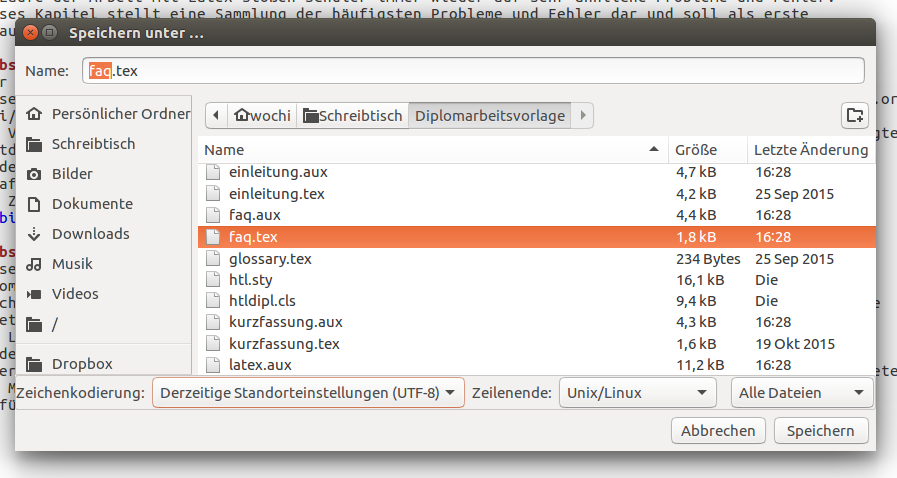
\includegraphics[width=.85\textwidth]{SpeichernUnter}
\caption{Speichern Unter Dialog mit der Auswahlmöglichkeit der Zeichenkodierung}
\label{fig:speichernunter}
\end{figure}

\subsubsection*{Beim Erzeugen des PDFs kommt eine Fehlermeldung das Paket XYZ.sty fehlt.}
Dieser Fehler hängt von der verwendeten Latex-Installation ab. Bei Miktex können fehlende Pakete automatisch nachinstalliert werden. 
Manchmal funktioniert diese Automatik jedoch nicht. In diesem Fall ist es am Einfachsten die fehlende Pakete im Miktex-Manager manuell zu installieren. 
Bei Linux und anderen Betriebssystemen kann die Latex-Umgebung meist als Full-Install installiert werden. Hier werden alle verfügbaren Pakete installiert. 
Alternativ kann man mit Google ermitteln welches Installationspaket\footnote{Übersicht der Latex-Pakete für Mac \url{https://trac.macports.org/wiki/TeXLivePackages}} die benötigen XYZ.sty Dateien zur Verfügung stellt.

\subsubsection*{Das Inhaltsverzeichnis, Glossar, Literaturverzeichnis, ... wird nicht mehr angezeigt.}
Wärend die einzelnen Kapitel der Vorlage in der Datei \textit{\_Diplomarbeitsvorlage.tex} problemlos gegen die eigenen Kapitel ausgetauscht werden können, sind die anderen Befehle in dieser Datei kritisch für ein funktionieren der Vorlage. Wurde hier aus Versehen eine falsche Zeile gelöscht oder verändert, kann dies unerwartete Auswirkungen haben. In dem Fall am Besten die eigene \textit{\_Diplomarbeitsvorlage.tex} mit der aus der Vorlage vergleichen und gegebenenfalls eigene Änderungen vorübergehen zurück nehmen bis der Fehler gefunden ist.
\chapter{Abbildungen, Tabellen, Quellkode}
\label{chap:Abbildungen}

\section{Allgemeines}

Abbildungen (\emph{figures}) und Tabellen (\emph{tables}) werden üblicherweise
zusammen mit einem nummerierten Titel (\emph{caption}) zentriert
angeordnet (siehe Abb.~\ref{fig:urlaub}).
Im Text \emph{muss} es zu jeder Abbildung einen Verweis geben und die eigentliche Abbildung
sollte erst \emph{nach} dem ersten Verweis platziert werden.

\begin{figure}
\centering
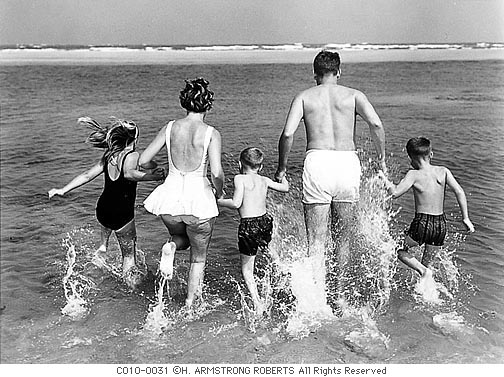
\includegraphics[width=.85\textwidth]{CS0031}
\caption{Newport Beach 1957.}
\label{fig:urlaub}
\end{figure}



\section{\emph{Let Them Float!}}

Das Platzieren von Abbildungen und Tabellen gehört zu den
schwierigsten Aufgaben im Schriftsatz, weil diese meist viel Platz
benötigen und häufig nicht auf der aktuellen Seite im laufenden
Text untergebracht werden können. Diese Elemente müssen daher an
eine geeignete Stelle auf nachfolgenden Seiten verschoben werden,
was manuell sehr mühsam (jedoch in \emph{Word} beispielsweise unerlässlich) ist.

In \latex funktioniert das weitgehend automatisch, indem
Abbildungen, Tabellen und ähnliche als "`Floating Bodies"'
behandelt werden. Bei der Positionierung dieser Elemente wird
versucht, einerseits im Textfluss möglichst wenig Leer\-raum
entstehen zu lassen und andererseits die Abbildungen und Tabellen
nicht zu weit von der ursprünglichen Textstelle zu entfernen.

Der Gedanke, dass etwa Abbildungen kaum jemals genau an der
ge\-wünsch\-ten Stelle und möglicherweise nicht einmal auf
derselben Seite Platz finden, ist für viele Anfänger aber offenbar sehr
ungewohnt oder sogar beängstigend. Dennoch sollte man zunächst einmal
getrost \latex\ diese Arbeit überlassen und \emph{nicht} manuell
eingreifen. Erst am Ende, wenn das gesamte Dokument "`steht"' und
man mit der automatischen Platzierung wirklich nicht zurande
kommt, sollte man (durch gezielte Platzierungsanweisungen
\cite[S.~33]{Oetiker01}) \textbf{in Einzelfällen} eingreifen.



\section{Captions}

Bei Abbildungen steht der Titel üblicherweise \emph{unten}, bei
Tabellen hingegen -- je nach Konvention -- \emph{oben} (wie in diesem Dokument) 
oder ebenfalls \emph{unten}. In \latex\ erfolgt
auch die Nummerierung der Abbildungen automatisch, ebenso der
Eintrag in das (optionale)
Abbildungsverzeichnis%
\footnote{Ein eigenes Verzeichnis der Abbildungen am Anfang des Dokuments
ist zwar leicht erstellt, in einer Diplomarbeit aber (und eigentlich
überall sonst auch) überflüssig. Man sollte es daher weglassen.}
am Beginn des Dokuments.

Die Markierung der Captions%
\footnote{Ausnahmsweise wird das Wort "`Caption"' im Folgenden
ohne deutsche Übersetzung verwendet.} erfolgt in \latex mithilfe
der \verb!\label{}! Anweisung, die unmittelbar auf die
\verb!\caption{}! Anweisung folgen muss:
%
\begin{LaTeXCode}
\begin{figure}
\centering
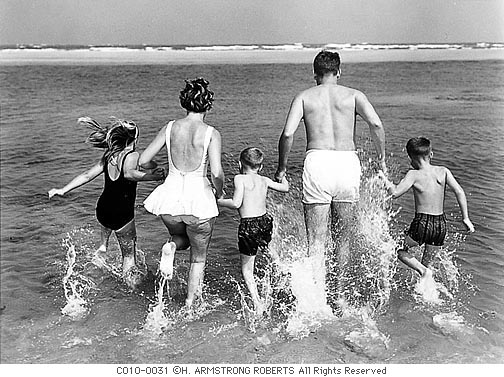
\includegraphics[width=.85\textwidth]{CS0031}
\caption{Newport Beach 1957.}
\label{fig:urlaub}
\end{figure}
\end{LaTeXCode}
%
Der Name des Labels (\texttt{fig:urlaub}) kann beliebig gewählt werden. 
Die Kennzeichnung \texttt{fig:} ist (wie in Abschn.\ \ref{sec:querverweise} 
erwähnt) nur eine nützliche Hilfe, um beim Schreiben verschiedene Arten 
von Labels besser unterscheiden zu können.

Die Länge der Captions kann dabei sehr unterschiedlich sein. Je
nach Anwendung und Stil ergibt sich manchmal eine sehr kurze
Caption (Abb.~\ref{fig:urlaub}) oder eine längere
(Abb.~\ref{fig:univac}).
Man beachte, wie bei kurzen Captions ein
zentrierter Satz und bei langen Captions ein Blocksatz verwendet
wird (\latex macht das automatisch).
Captions sollten \emph{immer} mit einem Punkt abgeschlossen sein.%
\footnote{Kurioserweise verlangen manche Anleitungen
genau das Gegegenteil, angeblich, weil beim klassischen Bleisatz 
die abschließenden Punkte im Druck häufig "`weggebrochen"' sind. 
Das kann man glauben oder nicht, im Digitaldruck 
spielt es jedenfalls keine Rolle.}

\begin{figure}
\centering
\FramePic{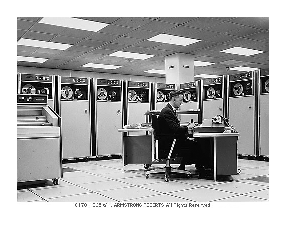
\includegraphics[width=.85\textwidth]{CS1065}}
\caption{Beispiel für einen langen Caption-Text. \textsc{Univac}
brachte 1961 mit dem Modell 751 den ersten Hochleistungsrechner
mit Halbleiterspeicher auf den Markt. Von diesem Computer wurden
in den U.S.A.\ bereits im ersten Produktionsjahr über fünfzig
Exemplare verkauft, vorwiegend an militärische Dienststellen,
Versicherungen und Großbanken. Die Ablöse erfolgte zwei Jahre
später durch das zusammen mit \textsc{Sperry} entwickelte Modell 820.
Das klingt vielleicht plausibel, ist aber frei erfunden und
vermutlich völliger Unsinn.} 
\label{fig:univac}
\end{figure}





\section{Abbildungen}

Für die Einbindung von Grafiken in \latex wird die Verwendung des Stan\-dard-Pakets
\texttt{graphicx}\footcite{Carlisle99} empfohlen 
(wird durch das \texttt{htl}-Paket bereits eingebunden). 
Folgende Bildformate können verwendet werden:
%
\begin{center}
\begin{tabular}{|l|l|l|}
\hline
Rasterbilder:    & PNG, JPEG, PDF \\
\hline
Vektorgraphiken: & PDF \\
\hline
\end{tabular}
\end{center}
%

\subsection{Wo liegen die Grafikdateien?} 

Die Bilder werden üblicherweise in einem Unterverzeichnis (oder in mehreren Unterverzeichnissen) abgelegt,
im Fall dieses Dokuments in \url{images/}.
Dazu dient die folgende Anweisung
am Beginn des Hauptdokuments \url{Diplomarbeit.tex} (\sa\ Anhang
\ref{app:latex}):
%
\begin{quote}\small
\verb!\graphicspath{{images/}}!
\end{quote}
%
Der (zum Hauptdokument relative) Pfad \texttt{graphicspath} kann innerhalb des
Dokuments jederzeit geändert werden, was durchaus nützlich ist, wenn man
\zB\ die Grafiken einzelner Kapitel getrennt in entsprechenden Verzeichnissen
ablegen möchte.
Die Größe der Abbildung im Druck kann durch Vorgabe einer bestimmten
Breite oder Höhe oder eines Skalierungsfaktors gesteuert werden, {\zB}:
%
\begin{quote}\small
\verb!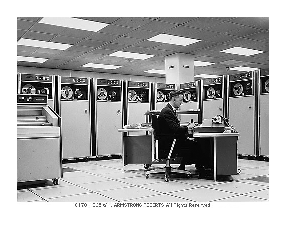
\includegraphics[width=.85\textwidth]{CS1065}! \\
\verb!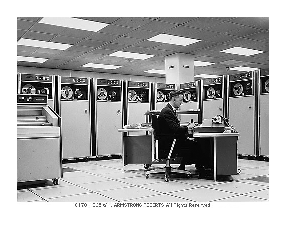
\includegraphics[scale=1.5]{CS1065}!
\end{quote}
%
Man beachte, dass dabei die Datei-Extension nicht explizit angegeben werden muss. 
Das ist \va\ dann praktisch, wenn man verschiedene Workflows mit jeweils
unterschiedlichen Dateitypen verwendet.


\subsection{Grafiken einrahmen} 

Mit dem Makro \verb!\FramePic{}! (definiert in \texttt{htl.sty}) kann man
optional einen dünnen Rahmen rund um die Grafik erzeugen, \zB:
%
\begin{quote}\small
\verb!\FramePic{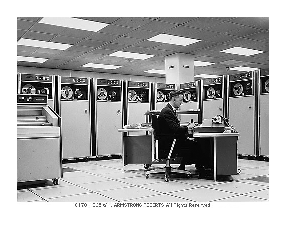
\includegraphics[height=50mm]{CS1065}}!
\end{quote}
%
Das wird man üblicherweise nur bei Rasterbildern tun, insbesondere wenn sie zum Rand hin sehr hell sind
und ohne Rahmen nicht vom Hintergrund abgrenzbar wären.

\subsection{Rasterbilder (Pixelgrafiken)}

Generell sollte man Bilder bereits vorher so aufbereiten,
dass sie später beim Druck möglichst wenig an Qualität verlieren.
Es empfiehlt sich daher, die Bildgröße (Auflösung) bereits im Vorhinein
(\zB mit \emph{Photoshop})
richtig einzustellen.
Brauchbare Auflösungen bezogen auf die endgültige Bildgröße sind:
%
\begin{itemize}
  \item \textbf{Farb- und Grauwertbilder:} 150--300 dpi
  \item \textbf{Binärbilder (Schwarz/Weiß):} 300--600 dpi
\end{itemize}
%
Eine wesentlich höhere Auflösung macht aufgrund der beim Laserdruck notwendigen
Rasterung keinen Sinn, auch bei 1200 dpi-Druckern.
Speziell \emph{Screen\-shots} sollte man nicht zu klein darstellen,
da sie sonst schlecht lesbar sind (max.\ 200 dpi, besser 150 dpi).
Dabei ist zu bedenken, dass die Arbeit auch als Kopie in allen
Details noch gut lesbar sein sollte.

\subsubsection{JPEG-Problematik}

Keinesfalls sollte man Bilder, die für den Einsatz in
Druckdokumenten gedacht sind, mit verlustbehafteten
Kompressionsverfahren abspeichern. Insbesondere sollte man die Verwendung
von JPEG möglichst vermeiden, auch wenn viele Dateien dadurch
wesentlich kleiner würden. 
Eine Ausnahme ist, wenn die Originaldaten nur in JPEG vorliegen und für die 
Einbindung nicht bearbeitet oder verkleinert wurden. Ansonsten sollte man immer
PNG verwenden.

Besonders gerne werden farbige \textbf{Screenshots} einer JPEG-Kompression%
\footnote{Das JPEG-Verfahren ist für natürliche Fotos konzipiert und dafür auch gut geeignet,
seine undifferenzierte Verwendung ist aber zu einer globalen Plage geworden.}
unterzogen, obwohl deren verheerende Folgen auch für jeden Laien sichtbar sein sollten
(Abb.~\ref{fig:jpeg-pfusch}).

\begin{figure}
\centering\small
\begin{tabular}{cc}
\FramePic{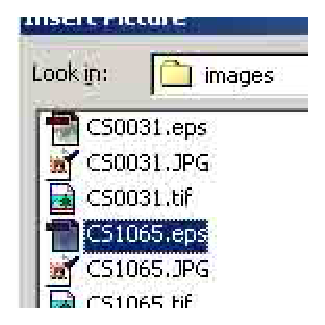
\includegraphics[width=0.45\textwidth]{screenshot-dirty}} &		% JPEG file
\FramePic{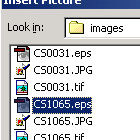
\includegraphics[width=0.45\textwidth]{screenshot-clean}} \\	% PNG file
(a) & (b) 
\end{tabular}
\caption{Typischer JPEG-Pfusch. Screenshots und ähnliche im Original
verfügbare Rasterbilder sollten für Druckdokumente \emph{keinesfalls} mit
JPEG komprimiert werden. Das Ergebnis (a) sieht gegenüber dem
unkomprimierten Original (b) nicht nur schmutzig aus, sondern wird
auch schnell unleserlich.} 
\label{fig:jpeg-pfusch}
\end{figure}






\subsection{Vektorgrafiken}

Für schematische Abbildungen (\zB Flussdiagramme, Entity-Relationship-Diagramme
oder sonstige strukturelle Darstellungen) sollte man unbedingt
Vektorgrafiken verwenden.
Gerasterte Grafiken, wie man sie üblicherweise als GIF- oder PNG-Dateien
auf Webseiten findet, haben in einem Druckdokument nichts zu suchen, notfalls
muss man sie mit einem entsprechenden Werkzeug \emph{neu} zeichnen (natürlich
unter Angabe der ursprünglichen Quelle).

In diesem Fall kommt als Datenformat nur PDF in Frage,
dieses bietet sich aber auch in anderen Umgebungen als universelles
Vektor-Format an.
Zur Erstellung von PDF-Vektorgrafiken benötigt man ein geeignetes
Grafikprogramm, \zB\ \emph{Freehand} von \emph{Macromedia}
oder \emph{Illustrator} von \emph{Adobe}.
Manche gängige Grafikprogramme 
unterstützen allerdings keinen direkten Export von PDF-Dateien
oder erzeugen unbrauchbare Dateien. Vor der Entscheidung
für eine bestimmte Zeichensoftware sollte man das im Zweifelsfall
ausprobieren.
PDF kann im Notfall über einen entsprechenden Druckertreiber erzeugt werden.




\subsubsection{Einbettung von Schriften}

Die Wiedergabe von Textelementen ist abhängig von der auf dem
Computer (oder Drucker) installierten Schriften und der Form der
Schrifteinbettung im Quelldokument. Die korrekte Darstellung am
Bildschirm eines Computers bedeutet nicht, dass dasselbe Dokument
auf einem anderen Computer oder Drucker genau so dargestellt wird.
Dieser Umstand ist besonders wichtig, wenn Druckdokumente online
zur Verfügung gestellt werden. Kontrollieren Sie daher genau, ob
die innerhalb Ihrer Grafiken verwendeten Schriften auch exakt wie
beabsichtigt im Ausdruck aufscheinen.


\subsubsection{Strichstärken -- \emph{Hairlines} vermeiden!}

In Grafik-Programmen wie \emph{Freehand} und \emph{Illustrator},
die sich im Wesentlichen an der \emph{PostScript}-Funktionalität
orientieren, ist es möglich, Linien bzgl.\ ihrer Stärke als
"`Hairline"' zu definieren. Im zugehörigen \emph{PostScript}-Kode
wird dies als \texttt{linewidth} mit dem Wert \texttt{0} ausgedrückt und
sollte am Ausgabegerät "`möglichst dünne"' Linien ergeben. Das
Ergebnis ist ausschließlich vom jeweiligen Drucker
abhängig und somit kaum verhersagbar. 
\textbf{Fazit:} Hairlines vermeiden und stattdessen immer konkrete
Strichstärken ($\geq 0.25 \mathrm{pt}$) einstellen!


\subsection{\tex-Schriften auch in Grafiken?}
\label{sec:tex-schriften-in-grafiken}

Während man sich bei Abbildungen, die mit externen
Grafik-Programmen erzeugt werden, meist mit ähnlich aussehenden
Schriften (wie \emph{Times-Roman} oder \emph{Garamond}) abhilft,
besteht bei Puristen oft der verständliche Wunsch, die 
\emph{Computer-Modern} (CM) Schriftfamilie von {\tex}/{\latex} auch
innerhalb von eingebetteten Grafiken einzusetzen.

\subsubsection{\emph{BaKoMa}-Schriften}

Glücklicherweise stehen einige Portierungen von CM als {\em
TrueType}-Schriften zur Verfügung, die man auch in herkömmlichen
DTP-Anwendungen unter \emph{Windows} und \emph{Mac~OS} verwenden
kann. Empfehlenswert ist \va\ die \emph{BaKoMa Fonts
Collection}\footnote{Von Basil K.\ Malyshev -- die BaKoMa-Fonts
liegen dieser Vorlage bei, ansonsten findet man sie \zB\ unter
\url{www.ctan.org/tex-archive/fonts/cm/ps-type1/bakoma/}.}, die
neben den CM-Standardschriften auch die mathematischen Schriften
der AMS-Familie ent\-hält und zudem kostenfrei ist. Natürlich
müssen die TrueType Schriften vor der Verwendung zunächst auf dem
eigenen PC installiert werden.


\subsection{Abbildungen mit mehreren Elementen}

Werden mehrere Bilder oder Grafiken zu einer Abbildung zusammengefasst, 
verwendet man üblicherweise eine gemeinsame Caption, wie in Abb.~\ref{fig:Bearings}
dargestellt. Im Text könnte ein Verweis auf einen einzelnen Teil der Abbildung, etwa das 
einreihige Rollenlager in Abb.~\ref{fig:Bearings}\thinspace(c), so aussehen:
%
\begin{itemize}
\item[] \verb!Abb.~\ref{fig:Bearings}\thinspace(c)! 
\end{itemize}
%
Für kompliziertere Abbildungen sollte man die Verwendung des 
\texttt{subfigure}-Pakets \footcite{Cochran95} in Betracht ziehen. Ein Beispiel ist in der Vorlage in Abbildung \ref{fig:Settings} zu finden.


\subsection{Quellenangaben in Captions}
\label{sec:QuellenangabenInCaptions}

Wenn Bilder, Grafiken oder Tabellen aus anderen Quellen verwendet werden, dann muss ihre Herkunft in jedem Fall klar ersichtlich gemacht werden, und zwar am besten direkt in der Caption.
Verwendet man beispielsweise eine Grafik aus einem Buch oder einer sonstigen zitierfähigen Publikation, dann sollte man diese in das Literaturverzeichnis aufnehmen und wie üblich zitieren, wie in Abb.\ \ref{fig:Bearings} demonstriert. Da Grafiken floating-Elemente sind, muss statt mit
\verb!\footcite{..}! die Kombination \verb!\footnotemark! und \verb!\footcitetext! verwendet werden. Weitere Details zu dieser Art von Quellenangaben finden sich in Kap.\ \ref{cha:Literatur}.

Bei Bildern aus dem Internet ist es hingegen ratsam, die zugehörige Website \emph{nicht} in das Literaturverzeichnis aufnehmen, sondern (mit \verb!\url{..}!) direkt in der Caption oder in einer Fußnote anzugeben (siehe Abschn.\ \ref{sec:OnlineQuellen} und Abbildung \ref{fig:latexinternet}). 

Sollte die Kombination von Caption, Fußnote und Url verwendet werden, muss die Fußnote in ein \verb!\footnotemark! und ein \verb!\footnotetext! aufgeteilt werden. Abbildung \ref{fig:latexinternet} zeigt ein Beispiel davon und das Programm \ref{prog:footnotemark} zeigt den \latex\ Quelltext. Die Fußnote wird in diesem Fall nicht immer auf der selben Seite wie die Abbildung sein, was durch die Durchnumerierung der Fußnoten jedoch kein Problem darstellen sollte. Vor allem, da die Fußnote sich dann auf der Seite befindet wo die Abbildung im Text erwähnt werden sollte. 

\begin{program}
% place caption consistently either at the top or bottom:
\caption{\latex\ Quelltext zu Abbildung \ref{fig:latexinternet}.}
\label{prog:footnotemark}
%
\begin{LaTeXCode}
\begin{figure}
\centering

\includegraphics[width=.85\textwidth]{LatexInternet}
\caption[]{Witze über Latex im Internet.\footnotemark }
\label{fig:latexinternet}
\end{figure}
\footnotetext{Quelle: \url{https://pr0gramm.com/static/1454890}}
\end{LaTeXCode}
%
\end{program}

% Beispiel für die Verwendung von "subfigure"

\begin{figure}
\centering\small
\begin{tabular}{cc}
  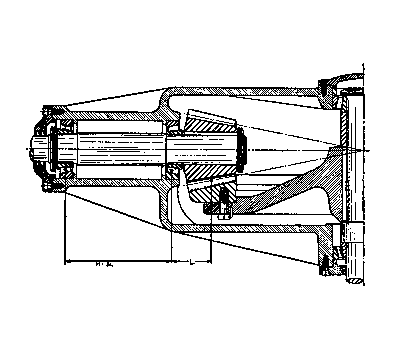
\includegraphics[width=.45\textwidth]{overhang-mounting} &
  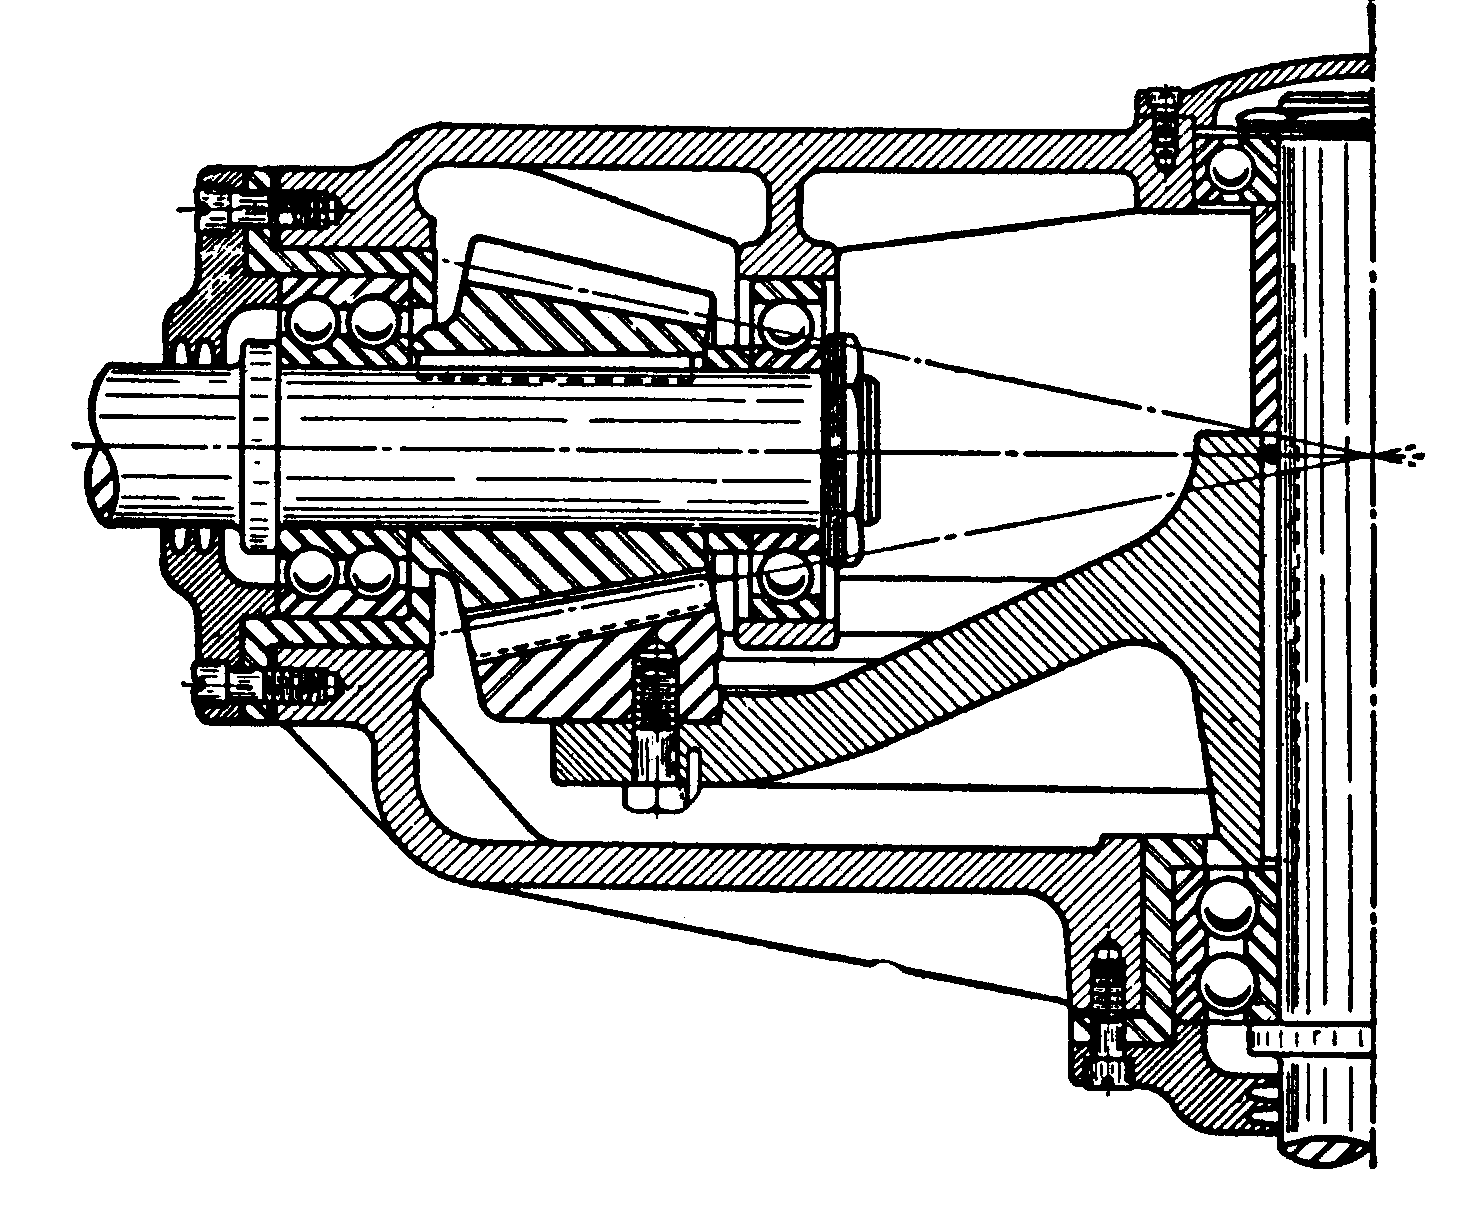
\includegraphics[width=.45\textwidth]{straddle-mounting} \\
  (a) & (b)
\\[4pt]	%vertical extra spacing (4 points)
  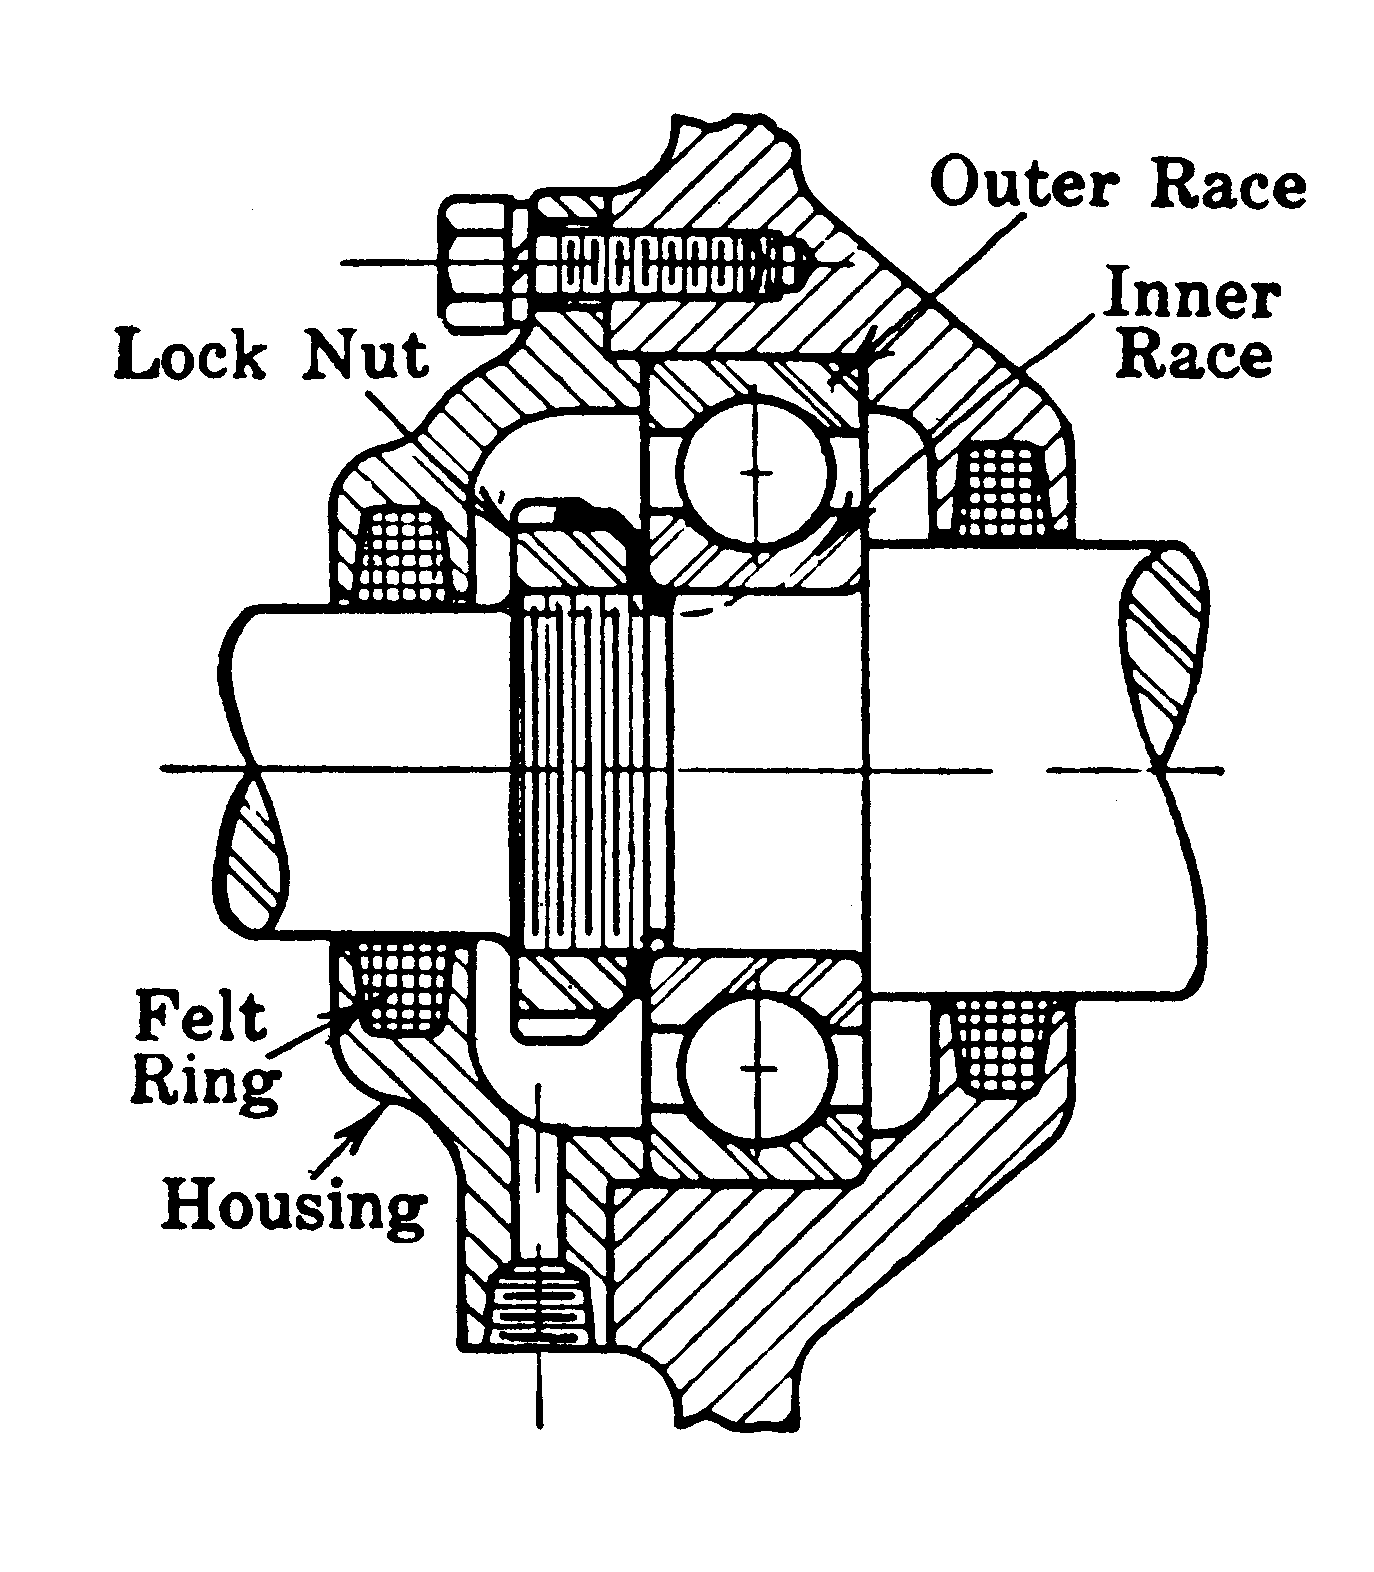
\includegraphics[width=.45\textwidth]{ball-bearing-1} &
  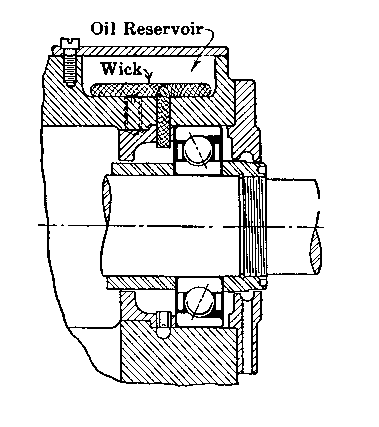
\includegraphics[width=.45\textwidth]{ball-bearing-2} \\
  (c) & (d)
\end{tabular}
%
\caption[]{Diverse Maschinenelemente.
Overhang Mounting (a), Straddle Mounting (b),
einreihiges Rollenlager (c), Schmierung von Rollenlagern (d).
Aus \citetitle{Faires34}.\footnotemark }
\label{fig:Bearings}
\end{figure}
\footcitetext{Faires34}

\begin{figure}
\centering

\includegraphics[width=.85\textwidth]{LatexInternet}
\caption[]{Witze über Latex im Internet.\footnotemark }
\label{fig:latexinternet}
\end{figure}
\footnotetext{Quelle: \url{https://pr0gramm.com/static/1454890}}

\section{Tabellen}

Tabellen werden häufig eingesetzt um numerische Zusammenhänge, Testergebnisse
etc.\ in übersichtlicher Form darzustellen.
Ein einfaches Beispiel ist Tab.~\ref{tab:processors}, der \latex-Quelltext dazu
findet sich in Prog.~\ref{prog:processors-source}.


\begin{table}
\caption{Prozessor-Familien im Überblick.}
\label{tab:processors}
\centering
\setlength{\tabcolsep}{5mm}	% separator between columns
\def\arraystretch{1.25}		% vertical stretch factor
\begin{tabular}{|r||c|c|c|} \hline
& \emph{PowerPC} & \emph{Pentium} & \emph{Athlon} \\
\hline\hline
Manufacturer & Motorola & Intel & AMD \\
\hline
Speed & high & medium & high   \\
\hline
Price & high & high   & medium \\
\hline
\end{tabular}
\end{table}

\begin{program}
% place caption consistently either at the top or bottom:
\caption{\latex\ Quelltext zu Tab.~\ref{tab:processors}.
Die Erzeugung des dargestellten Listings selbst ist in Abschn.\ \ref{sec:programmtexte} beschrieben.}
\label{prog:processors-source}
%
\begin{LaTeXCode}
\begin{table}
\caption{Prozessor-Familien im "Uberblick.}
\label{tab:processors}
\centering
\setlength{\tabcolsep}{5mm}	% separator between columns
\def\arraystretch{1.25}		% vertical stretch factor
\begin{tabular}{|r||c|c|c|} \hline
& \emph{PowerPC} & \emph{Pentium} & \emph{Athlon} \\
\hline\hline
Manufacturer & Motorola & Intel & AMD \\
\hline
Speed & high & medium & high   \\
\hline
Price & high & high   & medium \\
\hline
\end{tabular}
\end{table}
\end{LaTeXCode}
%
\end{program}

Manchmal ist es notwendig, in Tabellen relativ viel Text in engen Spalten
unter zu bringen, wie in Tab.~\ref{tab:synthesis-techniques}. In diesem Fall
ist es sinnvoll, auf den Blocksatz zu verzichten und gleichzeit die
strengen Abteilungsregeln zu lockern. Details dazu finden sich im zugehörigen
\latex-Quelltext.


%--------------------------------------------------------------------------------
% Table with narrow columns
%--------------------------------------------------------------------------------
\begin{table}
\caption{Beispiel für eine Tabelle mit mehrzeiligem Text in engen Spalten.
Hier werden die Zeilen für den Blocksatz zu kurz, daher wird linksbündig
gesetzt (im "`Flattersatz"').}
\label{tab:synthesis-techniques}
\centering
\def\rr{\rightskip=0pt plus1em \spaceskip=.3333em \xspaceskip=.5em\relax}
\setlength{\tabcolsep}{1ex}
\def\arraystretch{1.20}
\setlength{\tabcolsep}{1ex}
\small
\begin{english}
\begin{tabular}{|p{0.2\textwidth}|c|p{0.3\textwidth}|p{0.2\textwidth}|}
\hline
   \multicolumn{1}{|c}{\emph{Method}} &
   \multicolumn{1}{|c}{\emph{Implem.}} &
   \multicolumn{1}{|c}{\emph{Features}} &
   \multicolumn{1}{|c|}{\emph{Status}} \\
\hline\hline
   {\rr polygon shading} &
   SW/HW &
   {\rr flat-shaded polygons} &
   \\
\hline
  {\rr flat shading with z-buffer} &
  SW/HW &
  {\rr depth values} &
  \\
\hline
  {\rr goraud shading with z-buffer} &
  SW/HW &
  {\rr smooth shading, simple fog, point light sources} &
  {\rr SGI entry models} \\
\hline
  {\rr phong shading with z-buffer} &
  SW/HW &
  {\rr highlights} &
  \\
\hline
  {\rr texture mapping with z-buffer} &
  SW/HW &
  {\rr surface textures, simple shadows} &
  {\rr SGI high end, flight simulators} \\
\hline
%  {\rr reflection mapping with z-buffer} &
%  SW/HW &
%  {\rr reflections} &
%  {\rr SGI next generation} \\
%\hline
%  {\rr raytracing} &
%  SW &
%  {\rr refraction, real camera model, area light sources with penumbra, realistic material models} &
%  {\rr common ray\-tracers} \\
%\hline
%  {\rr raytracing + global illumination simulation} &
%  SW &
%  {\rr indirect illumination} &
%  \textit{Radiance} \\
%\hline
%  {\rr raytracing + global illumination simulation + dissipating media} &
%  none &
%  {\rr realistic clouds, scattering, ...} &
%  {\rr research} \\
%\hline
\end{tabular}
\end{english}
\end{table}

%--------------------------------------------------------------------------------



\section{Programmtexte}
\label{sec:programmtexte}

Die Einbindung von Programmtexten (source code) ist eine häufige Notwendigkeit,
\va natürlich bei Arbeiten im Bereich der Informatik.

\subsection{Formatierung von Programmkode}
\label{sec:FormatierungVonProgrammkode}

Es gibt für \latex\ spezielle Pakete zur Darstellung von Programmen, die \ua\
auch die automatische Nummerierung der Zeilen vornehmen. Zu empfehlen ist hier
insbesondere das \texttt{listings2}-Package\footnote{Aktuell noch als
Beta-Version, ist notwendig zur Unterstützung von UTF-8.}. In \texttt{htl.sty}
sind damit folgende Umgebungen definiert:
%
\begin{center}
\begin{tabular}{ll}
C (ANSI):   & \verb!\begin{CCode}       ... \end{CCode}! \\
C++ (ISO):  & \verb!\begin{CppCode}     ... \end{CppCode}! \\
Java:       & \verb!\begin{JavaCode}    ... \end{JavaCode}! \\
\latex:     & \verb!\begin{LaTeXCode}   ... \end{LaTeXCode}! \\
PHP:  		& \verb!\begin{PhpCode}     ... \end{PhpCode}! \\
Python:  	& \verb!\begin{PythonCode}  ... \end{PythonCode}! \\
C\#:  		& \verb!\begin{CSharpCode}  ... \end{CSharpCode}! \\
Generisch:  & \verb!\begin{GenericCode} ... \end{GenericCode}! 
\end{tabular}
\end{center}
%
Der Quellkode innerhalb dieser Umgebungen wird in der jeweiligen Programmiersprache interpretiert, wobei Kommentare erhalten bleiben. Diese Umgebungen können sowohl alleinstehend (im Fließtext) oder innerhalb von Float-Umgebungen (insbes.\ \texttt{program}) verwendet werden. Im ersten Fall wird der Quelltext auch über Seitengrenzen umgebrochen. Mit \verb!/+! ... \verb!+/! ist eine Escape-Möglichkeit nach \latex\ vorgesehen, die \va\ zum Setzen von Labels für Verweise auf einzelne Programmzeilen nützlich ist, \zB
%
\begin{quote}
\verb!/+ \label{ExampleCodeLabel} +/!
\end{quote}
%
Ein Beispiel mit Java ist in Prog.~\ref{prog:CodeExample} gezeigt, wobei der oben angeführte Label in Zeile \ref{ExampleCodeLabel} steht.
Man beachte, dass innerhalb der Kommentare auch mathematischer Text (wie etwa in Zeile \ref{MathInCode} von Prog.~\ref{prog:CodeExample}) stehen kann.

\begin{program}
% place caption consistently either at the top or bottom:
\caption{Beispiel für die Auflistung von Programmkode als Float-Element.}
\label{prog:CodeExample}
\begin{JavaCode}
import ij.ImagePlus;
import ij.plugin.filter.PlugInFilter;
import ij.process.ImageProcessor;

public class My_Inverter implements PlugInFilter {

  String title = ""; // just to test printing of double quotes

	public int setup (String arg, ImagePlus im) {
		return DOES_8G;	// this plugin accepts 8-bit grayscale images \label{pr:IjSamplePlugin10}
	}

	public void run (ImageProcessor ip) {
		int w = ip.getWidth();	/+ \label{ExampleCodeLabel} +/
		int h = ip.getHeight(); 
		
		/* iterate over all image coordinates */
		for (int u = 0; u < w; u++) { 
			for (int v = 0; v < h; v++) {
				int p = ip.getPixel(u, v); 
				ip.putPixel(u, v, 255-p); // invert: $I'(u,v) \leftarrow 255 - I(u,v)$\label{MathInCode}
			}
		}
	}
			
} // end of class {\tt My\_Inverter}
\end{JavaCode}
%
\end{program}


\subsection{Platzierung von Programmkode}

Da Quelltexte sehr umfangreich werden können, ist diese Aufgabe nicht
immer leicht zu lösen. Abhängig vom Umfang und vom Bezug zum Haupttext
gibt es grundsätzlich drei Möglichkeiten zur Einbindung von Programmtext:
%
\begin{itemize}
\item[a)] im laufenden Text für kurze Programmstücke,
\item[b)] als Float-Element (\texttt{program}) für mittlere Programmtexte bis max.\ eine Seite oder
\item[c)] im Anhang (für lange Programmtexte).
\end{itemize}

\subsubsection{Programmtext im laufenden Text}

Kurze Kodesequenzen kann man ohne weiteres im laufenden Text
einbetten, sofern sie an den gegebenen Stellen von unmittelbarer
Bedeutung sind. Die folgende (rudimentäre) Java-Methode {\tt
extractEmail} sucht nach einer E-Mail Adresse in der Zeichenkette
\texttt{line}:

\medskip
\begin{JavaCode}
static String extractEmail(String line) {
    line = line.trim(); // find the first blank
    int i = line.indexOf(' '); 
    if (i > 0)
        return line.substring(i).trim();
    else
        return null;
}
\end{JavaCode}
\medskip

\noindent
Dieses Kodestück wurde mit 
\begin{quote}
\begin{verbatim}
\begin{JavaCode}
static String extractEmail(String line) {
    line = line.trim(); // find the first blank
    ...
}
\end{JavaCode}
\end{verbatim}
\end{quote}
erstellt (siehe Abschn.\ \ref{sec:FormatierungVonProgrammkode}). In-line Programmstücke sollten maximal einige Zeilen lang sein und nach Möglichkeit nicht durch Seitenumbrüche geteilt werden.
Um auch längere Programmzeilen unterzubringen, empfiehlt es sich, dafür
eine entsprechend kleine Schriftgröße zu wählen (als Standardgröße ist
\texttt{footnotesize} eingestellt). 



\subsubsection{Programmtexte als Float-Elemente}
Sind längere Kodesequenzen notwendig, die in unmittelbarer Nähe des laufenden Texts
stehen müssen, sollte man diese genauso wie andere Abbildungen als Float-Elemente
behandeln. Diese Programmtexte sollten den Umfang von einer Seite nicht übersteigen.
Im Notfall kann man auch bis zu zwei Seiten in aufeinanderfolgende Abbildungen packen,
jeweils mit eigener Caption. In \texttt{htl.sty} ist eine neue Float-Umgebung
\texttt{program} definiert, die analog zu \texttt{table} verwendet wird:
%
\begin{quote}
\begin{verbatim}
\begin{program}
\caption{Der Titel zu diesem Programmstück.}
\label{prog:xyz}
\begin{JavaCode}
  class IrgendWas {
    ...
  }
\end{JavaCode}
\end{program}
\end{verbatim}
\end{quote}
%
Wenn man möchte, kann man in diesem Fall die Caption auch unten anbringen (aber konsistent und nicht gemischt).
Natürlich darf man auch hier  nicht mit einer linearen  Abfolge im fertigen
Druckbild rechnen, daher sind Wendungen wie
"`... im  folgenden Programmstück ..."' zu vermeiden und entsprechende Verweise
einzusetzen. Beispiele dafür sind die Programme \ref{prog:processors-source} und \ref{prog:CodeExample}.


\subsubsection{Programmtext im Anhang}

Für längere Programmtexte, speziell wenn sie vollständige
Implementierungen umfassen und im aktuellen Kontext nicht
unmittelbar relevant sind, muss man zur Ablage in einem getrennten
Anhang am Ende des Dokuments greifen. Für Hinweise auf bestimmte
Details kann man entweder kurze Ausschnitte in den laufenden Text
stellen oder mit entsprechenden Seitenverweisen arbeiten. Ein
solches Beispiel ist der \latex-Quellkode in Anhang
\ref{app:latex} (Seite \pageref{app:latex}).%
\footnote{%
Grundsätzlich ist zu überlegen, ob die gedruckte Einbindung der gesamten
Programmtexte einer Implementierung für den Leser überhaupt sinnvoll ist, oder
ob man diese nicht besser elektronisch (auf CD-ROM) beifügt und nur exemplarisch
beschreibt.}

\chapter[Mathem.\ Formeln etc.]{Mathematische Formeln, Gleichungen und Algorithmen}
\label{chap:Mathematik}



Das Formatieren von mathematischen Elementen gehört sicher zu den
Stär\-ken von \latex. Man unterscheidet zwischen mathematischen Elementen
im Fließtext und freistehenden Gleichungen, die in der Regel
fortlaufend nummeriert werden. Analog zu Abbildungen und Tabellen sind dadurch
Querverweise zu Gleichungen leicht zu realisieren.
Hier nur einige Beispiele und spezielle Themen, vieles weitere dazu findet sich \zB in
\cite[Kap.\ 5]{Kopka98} oder \cite{mathmode09}.


\section{Mathematische Elemente im Fließtext}

Mathematische Symbole, Ausdrücke, Gleichungen etc.\ werden im Fließtext durch paarweise \verb!$! \ldots \verb!$! markiert. Hier ein Beispiel:
%
\begin{quote}
Der Nah-Unendlichkeitspunkt liegt bei
$\bar{a} = f' \cdot \bigl( \frac{f'}{K \cdot u_{\max}} + 1 \bigr)$,
sodass bei einem auf $\infty$ eingestellten Objektiv von der Entfernung
$\bar{a}$ an alles scharf ist. Fokussiert man das
Objektiv auf die Entfernung $\bar{a}$ (\dah, $a_0 = \bar{a}$), dann wird
im Bereich $[\frac{\bar{a}}{2}, \infty]$ alles scharf.
\end{quote}
%
Dabei sollte man unbedingt darauf achten, dass die Höhe der einzelnen Elemente im Text nicht zu groß wird. 

\paragraph{Häufiger Fehler:} 
Im Fließtext wird bei einfachen Variablen oft auf die Verwendung der richtigen, mathematischen Zeichen vergessen, wie etwa in 
"`X-Achse"' anstelle von "`$X$-Achse"' (\verb!$X$-Achse!).



\section{Freigestellte Ausdrücke}

Freigestellte mathematische Ausdrücke können in \latex\ im einfachsten Fall durch paarweise \verb!$$! \ldots \verb!$$! erzeugt werden. Das Ergebnis wird zentriert, erhält jedoch keine Numerierung. So ist \zB\ $$ y = 4 x^2 $$ das Ergebnis von \verb!$$ y = 4 x^2 $$!.

\subsection{Einfache Gleichungen} 

Meistens verwendet man in solchen Fällen jedoch die \texttt{equation}-Umgebung zur Herstellung numerierter Gleichungen, auf die man im Text jederzeit verweisen kann. Zum Beispiel erzeugt
%
\begin{LaTeXCode}
\begin{equation}
  f(k) = \frac{1}{N} \sum_{i=0}^{k-1} i^2 . 
  \label{eq:MyFirstEquation}
\end{equation}
\end{LaTeXCode}
%
die Gleichung
%
\begin{equation}
  f(k) = \frac{1}{N} \sum_{i=0}^{k-1} i^2 . 
\label{eq:MyFirstEquation}
\end{equation}
%
Mit \verb!\ref{eq:MyFirstEquation}! erhält man wie üblich die Nummer (\ref{eq:MyFirstEquation}) dieser Gleichung (siehe dazu auch Abschn.\ \ref{sec:VerweiseAufGleichungen}). 
Dieselbe Gleichung \emph{ohne} Numerierung kann man übrigens mit der \texttt{equation*}-Umgebung erzeugen.



\begin{center}
\setlength{\fboxrule}{0.2mm}
\setlength{\fboxsep}{2mm}
\fbox{%
\begin{minipage}{0.9\textwidth}
Man beachte, dass \textbf{Gleichungen} inhaltlich ein \textbf{Teil des Texts} sind und daher neben der sprachliche \textbf{Überleitung} auch die \textbf{Punktuation} (wie in Gl.\ \ref{eq:MyFirstEquation} gezeigt) beachtet werden muss. Bei Unsicherheiten sollte man sich passende Beispiele in einem guten Mathematik\-buch ansehen.
\end{minipage}}
\end{center}
%
Für Interessierte findet sich mehr zum Thema Mathematik und Prosa in \cite{Mermin89} und \cite{Higham98}.

\subsection{Mehrzeilige Gleichungen}

Für mehrzeilige Gleichungen bietet \latex\ die 
\verb!eqnarray!-Umgebung, die allerdings etwas eigenwillige Zwischenräume erzeugt.
Es empfiehlt sich, dafür gleich auf die erweiterten Möglichkeiten des \texttt{amsmath}-Pakets%
\footnote{American Mathematical Society (AMS). \texttt{amsmath} ist Teil der \latex\ Standardinstallation und wird von \texttt{htl.sty} bereits importiert.}
\cite{amsldoc02} zurückzugreifen.
Hier ein Beispiel mit zwei am \texttt{=}-Zeichen ausgerichteten Gleichungen,
%
\begin{align}
f_1 (x,y) &= \frac{1}{1-x} + y , \label{eq:f1} \\
f_2 (x,y) &= \frac{1}{1+y} - x , \label{eq:f2}
\end{align}
%
erzeugt mit der \texttt{align}-Umgebung aus dem \texttt{amsmath}-Paket:
%
\begin{LaTeXCode}
\begin{align}
  f_1 (x,y) &= \frac{1}{1-x} + y , \label{eq:f1} \\
  f_2 (x,y) &= \frac{1}{1+y} - x , \label{eq:f2}
\end{align}
\end{LaTeXCode}


\subsection{Fallunterscheidungen}

Mit der \texttt{cases}-Umgebung aus \texttt{amsmath} sind Fallunterscheidungen, \ua\ innerhalb von Funktionsdefinitionen, sehr einfach zu bewerkstelligen. Beispielsweise wurde die rekursive Definition
%
\begin{equation}
\mathsf{H}(i) =
\begin{cases}
  \mathsf{h}(0)                 & \text{für $i = 0$},\\
  \mathsf{H}(i-1) + \mathsf{h}(i) & \text{für $0 < i \leq K$}.
\end{cases}
\end{equation}
mit folgenden Anweisungen erzeugt:
%
\begin{LaTeXCode}
\begin{equation}
\mathsf{H}(i) =
\begin{cases}
  \mathsf{h}(0) & \text{f"ur $i = 0$},\\
  \mathsf{H}(i-1) + \mathsf{h}(i) & \text{f"ur $0 < i \leq K$}.
\end{cases}
\end{equation}
\end{LaTeXCode}
%
Man beachte dabei die Verwendung des sehr praktischen \verb!\text{..}!-Makros, mit dem im Mathematik-Modus gewöhnlicher Text eingefügt werden kann, sowie wiederum die Punktuation innerhalb der Gleichung.

\subsection{Gleichungen mit Matrizen}

Auch hier bietet \texttt{amsmath} einige Vorteile gegenüber der Verwendung der \latex\ Standardkonstrukte. Dazu ein einfaches Beispiel für die Verwendung der \texttt{pmatrix}-Umgebung für Vektoren und Matrizen,
%
\begin{equation}
\begin{pmatrix} x' \\ y' \end{pmatrix}
= 
\begin{pmatrix}
  \cos \phi & -\sin \phi \\
  \sin \phi & \phantom{-}\cos \phi
\end{pmatrix} 
\cdot
\begin{pmatrix}	x \\ y \end{pmatrix} ,
\end{equation}
%
das mit den folgenden Anweisungen erzeugt wurde:
%
\begin{LaTeXCode}
\begin{equation}
\begin{pmatrix} 
		x' \\ 
		y' 
\end{pmatrix}
= 
\begin{pmatrix}
	  \cos \phi & -\sin \phi \\
	  \sin \phi & \phantom{-}\cos \phi /+ \label{lin:phantom} +/
\end{pmatrix} 
\cdot
\begin{pmatrix} 
		x \\ 
		y 
\end{pmatrix} ,
\end{equation}
\end{LaTeXCode}
%
Ein nützliches Detail darin ist das \tex-Makro \verb!\phantom{..}! (in Zeile \ref{lin:phantom}), das sein Argument unsichtbar einfügt und hier als Platzhalter für das darüberliegende Minuszeichen verwendet wird. Alternativ kann man mit der \texttt{bmatrix}-Umgebung Matrizen mit eckigen Klammern erzeugen.
Zahlreiche weitere mathematische Konstrukte des \texttt{amsmath}-Pakets sind in \cite{amsldoc02} beschrieben.

\begin{comment}
% Umsetzung ohne amsmath:
\begin{equation}
\left[ \begin{array}{c}
  x' \\ y'
\end{array} \right] 
= 
\left[ \begin{array}{rr}
	 \cos \phi & \sin \phi \\
	-\sin \phi & \cos \phi
\end{array} \right] 
\cdot
\left[ \begin{array}{c}
	x \\ y
\end{array}
\right] 
.
\end{equation}
\end{comment}



\subsection{Verweise auf Gleichungen}
\label{sec:VerweiseAufGleichungen}

Beim Verweis auf nummerierte Formeln und Gleichungen genügt grundsätzlich die Angabe 
der entsprechenden Nummer in runden Klammern,
\zB\
\begin{center}
"`\ldots wie aus (\ref{eq:f1}) abgeleitet werden
kann \ldots"'
\end{center}
Um Missverständnisse zu vermeiden, sollte man aber -- \va\ in Texten mit
nur wenigen mathematischen Elementen -- "`Gleichung \ref{eq:f1}"', "`Gl.~\ref{eq:f1}"' oder "`Gl.~(\ref{eq:f1})"' schreiben (natürlich konsistent). 
%\emph{Falsch} wäre hingegen "`Gleichung (\ref{eqn:zerstreuungskreis})"'.

\begin{center}
\setlength{\fboxrule}{0.2mm}
\setlength{\fboxsep}{2mm}
\fbox{%
\begin{minipage}{0.9\textwidth}
\textbf{Achtung:} Vorwärtsverweise auf (im Text weiter hinten liegende) Gleichungen sind \textbf{äußerst ungewöhnlich} 
und sollten vermieden werden! Glaubt man dennoch so etwas zu benötigen, dann wurde
meistens ein Fehler in der Anordnung gemacht.
\end{minipage}}
\end{center}


\section{Spezielle Symbole}

\subsection{Zahlenmengen}
Einige häufig verwendete Symbole sind leider im ursprünglichen
mathematischen Zeichensatz von \latex nicht enthalten, \zB die
Symbole für die reellen und natürlichen Zahlen. Im {\tt
htl}-Paket sind diese Symbole als Makros \verb!\R! ($\R$),
\verb!\Z! ($\Z$), \verb!\N! ($\N$), \verb!\C! ($\C$) und \verb!\Q!
($\Q$)
mithilfe der \emph{AMS Blackboard Fonts} definiert, \zB:
\begin{center}
$x \in \R$ , $i \in \N_0$, $z \in \C$.
\end{center}


\subsection{Operatoren}

In \latex\ sind Dutzende von mathematischen Operatoren für spezielle Anwendungen definiert. Am häufigsten werden natürlich die arithmetischen Operatoren $+$, $-$, $\cdot$ und $/$ benötigt. Ein dabei oft beobachteter Fehler (der wohl aus der Programmierpraxis resultiert) ist die Verwendung von $*$ für die einfache Multiplikation -- richtig ist $\cdot$ (\verb!\cdot!).%
\footnote{Das Zeichen $*$ wird üblicherweise für den Faltungsoperator verwendet.}
%
Für Angaben wie \zB\ "`ein Feld mit $25 \times 70$ Metern"' (aber auch fast \emph{nur} dafür) verwendet man sinnvollerweise den $\times$ (\verb!\times!) Operator und \emph{nicht} einfach den Buchstaben "`x"'.


\subsection{Symbole mit mehreren Zeichen}
Vor allem bei der mathematischen Spezifikation von Algorithmen und Programmen
ist es häufig notwendig, Symbole (Variablennamen) mit mehr als einem Zeichen
zu verwenden, \zB
%
$$Scalefactor\leftarrow Scalefactor^2 \cdot 1.5 \; ,$$
%
erzeugt durch \verb!$Scalefactor! \verb!\leftarrow! \verb!Scalefactor^2! \verb!\cdot 1.5$!.
Dabei interpretiert \latex allerdings die Zeichenkette "`Scalefactor"' als 11 einzelne,
aufeinanderfolgende Symbole $S$, $c$, $a$, $l$, $e$, \ldots und setzt dazwischen
entsprechende Abstände.
Richtig ist, diese Buchstaben mit
\verb!\mathit{..}! zu \emph{einem} Symbol zusammenzufassen.
Der Unterschied ist in diesem Fall deutlich sichtbar:
%
\begin{center}
\setlength{\tabcolsep}{4pt}
\begin{tabular}{llll}
\text{Falsch:}   & $Scalefactor^2$ & $\leftarrow$ & \verb!$Scalefactor^2$! \\
\text{Richtig:}  & $\mathit{Scalefactor}^2$ & $\leftarrow$ & \verb!$\mathit{Scalefactor}^2$!
\end{tabular}
\end{center}
%
Grundsätzlich sollte man aber derart lange Symbolnamen ohnehin vermeiden und stattdessen möglichst einzelne 
Symbole verwenden
(\zB\ Brennweite $f = 50 \, \mathrm{mm}$ statt $\mathit{Brennweite} = 50 \, \mathrm{mm}$).

\subsection{Funktionen}

Während Symbole für Variablen traditionell (und in \latex\ automatisch) \emph{italic} gesetzt werden,
verwendet man für die Namen von Funktionen und Operatoren üblicherweise
\emph{roman} als Schrifttyp, wie \zB in
\begin{center}
\begin{tabular}{lcl}
$\sin \theta = \sin(\theta + 2 \pi)$ & & \verb!$\sin \theta = \sin(\theta + 2 \pi)$! \\
\end{tabular}
\end{center}
Das ist bei den bereits vordefinierten Standardfunktionen (wie
\verb!\sin!,
\verb!\cos!,
\verb!\tan!,
\verb!\log!,
\verb!\max!
\uva) automatisch der Fall.
Diese Konvention sollte man auch bei selbstdefinierten Funktionen befolgen,
wie etwa in
\begin{center}
\begin{tabular}{lcl}
$\mathrm{Distance}(A,B) = |A-B|$ & & \verb!$\mathrm{Distance}(A,B) = |A-B|$! \\
\end{tabular}
\end{center}


\subsection{Maßeinheiten und Währungen}

Bei der Angabe von Maßeinheiten wird üblicherweise Normalschrift
(keine Italics) verwendet, \zB:
\begin{quote}
Die Höchstgeschwindigkeit der \textit{Bell XS-1} beträgt 345~m/s
bei einem Startgewicht von 15~t. 
Der Prototyp kostete über 25{\thinspace}000{\thinspace}000 US\$, also ca.\ 19{\thinspace}200{\thinspace}000 \euro\ nach heutiger Umrechnung.
\end{quote}
Der Abstand zwischen der Zahl und der Maßeinheit ist dabei
gewollt.
Das \$-Zeichen erzeugt man mit \verb!\$!, während
das Euro-Symbol (\euro) nicht im ursprünglichen \latex-Zeichensatz enthalten ist. Es wird 
durch das Makro \verb!\euro! %\footnote{Aus dem \texttt{eurosym}-Paket.}
zur Verfügung gestellt.
Die kleinen Abstände zwischen den Ziffernblöcken der Beträge wurden hier übrigens mit \verb!{\thinspace}! erzeugt.



\subsection{Kommas in Dezimalzahlen (Mathematik-Modus)}

\latex\ setzt im Mathematik-Modus (also innerhalb von \verb!$$! oder in Gleichungen) nach dem anglo-merikanischen Stil in Dezimalzahlen grundsätzlich den \emph{Punkt} (\verb!.!) als Trennsymbol voraus. So wird etwa mit \verb!$3.141$! normalerweise die Ausgabe "`3.141"' erzeugt. Um das in Europa übliche Komma in Dezimalzahlen zu verwenden, genügt es \emph{nicht}, einfach \verb!.! durch \verb!,! zu ersetzen. Letzteres würde als Satzzeichen interpretiert und sieht dann so aus:
\begin{quote}
\verb!$3,141$!	$\quad \rightarrow \quad 3,141$ 
\end{quote}
(beachte den Leerraum nach dem Komma). Dieses Verhalten lässt sich in \latex\ zwar global umdefinieren, was aber wiederum zu einer Reihe unangenehmer Nebeneffekte führt. Eine einfache (wenn auch nicht sehr elegante) Lösung ist, Kommazahlen im Mathematik-Modus so zu schreiben:
\begin{quote}
\verb!$3{,}141$!	$\quad \rightarrow \quad 3{,}141$
\end{quote}



\subsection{Mathematik-Werkzeuge}

Für die Erstellung komplizierter Gleichungen ist es mitunter
hilfreich, auf spezielle Software zurückzugreifen. Unter anderem kann man
aus dem Microsoft \emph{Equation Editor} und aus {\em
Mathematica} auf relativ einfache Weise \latex-An\-wei\-sun\-gen
für mathematische Gleichungen exportieren und direkt (mit etwas
manueller Nacharbeit) in das eigene \latex-Dokument übernehmen.


\section{Algorithmen}

Für die Beschreibung von Algorithmen in mathematischer Form oder
Pseudo\-code ist in \latex selbst keine spezielle Unterstützung vorgesehen.
Dazu gibt es jedoch eine Reihe von \latex-Paketen (\zB\ \texttt{algorithms}, 
\texttt{algorithmicx}, \texttt{algorithm2e}).
Das Beispiel in Alg.~\ref{alg:xyz} wurde mit der Float-Umgebung von \texttt{algorithm} und dem algorithmischen Schriftsatz aus \texttt{algorithmicx} ausgeführt.%
\footnote{Hier wird \texttt{algorithmicx} \bzw\ \texttt{algpseudocode} in der älteren Version 1.1 verwendet (die zugehörigen \texttt{.sty}-Dateien liegen dieser Vorlage bei), weil die aktuelle Version (1.2) offenbar fehlerhaft ist. Als Alternative sollte man sich eventuell das \texttt{algorithm2e}-Paket ansehen.}
Die grobe Struktur dieses Konstrukts ist
%
\begin{LaTeXCode}
\begin{algorithm}
\caption{Bikubische Interpolation in 2D.}
\label{alg:xyz}
\begin{algorithmic}[1] 
  \Procedure{BicubicInterpolation}{$I, x_0, y_0$}
  ...
  \EndProcedure
\end{algorithmic}
\end{algorithm}
\end{LaTeXCode}

Weitere Details finden sich im Quelltext und natürlich in der Dokumentation der verwendeten Pakete.
Umfangreichere Beispiele für Algorithmen mit diesem Setup findet man \ua\ in \cite{BurgerBurge06}.


\begin{algorithm}
\caption{Bikubische Interpolation in 2D.}
\label{alg:xyz}
\smallskip
%
\begin{algorithmic}[1] % [1] heißt alle Zeilen werden numeriert
\Procedure{BicubicInterpolation}{$I, x_0, y_0$} \Comment{$x_0,y_0 \in \R$}
\Statex{Returns the interpolated value of the image $I$ 
        at the continuous position $(x_0, y_0)$.}
\State $q \gets 0$
\For{$j \gets 0 \ldots 3$} \Comment{iterate over 4 lines}
	\State $v \gets \lfloor y_0 \rfloor - 1 + j$
	\State $p \gets 0$ 
	\For{$i \gets 0 \ldots 3$} \Comment{iterate over 4 columns}
	  \State $u \gets \lfloor x_0 \rfloor - 1 + i$
	  \State $p \gets p + I(u,v) \cdot w_{\mathrm{cub}}(x_0 - u )$ 
	\EndFor
	\State $q \gets q + p \cdot w_{\mathrm{cub}}(y_0 - v)$
\EndFor
\State \textbf{return} $q$.
\EndProcedure
\end{algorithmic}%
\smallskip
%
\end{algorithm}
\chapter[Umgang mit Literatur]{Umgang mit Literatur und anderen Quellen}
\label{cha:Literatur}


\paragraph{Anmerkung:}
Der Titel dieses Kapitels ist für die Kopfzeile (absichtlich) zu
lang geraten; in diesem Fall kann man in der {\tt
chapter}-Anweisung von \latex als optionales Argument \verb![..]! einen verkürzten Text für die
Kopfzeile angeben:
\begin{verbatim}
  \chapter[Umgang mit Literatur]
          {Umgang mit Literatur und anderen Quellen}
\end{verbatim}

\section{Allgemeines}

Für die Gestaltung der Literaturverweise im Text und der
Quellenangaben sind weltweit eine Vielzahl verschiedener Richtlinien in
Gebrauch. Die Wahl des richtigen Schemas ist Geschmacksache -- wichtig ist jedoch,
eine durchdachte und vor allem \emph{konsistente} Verwendung.
Das Literaturverzeichnis ist eine
Zusammenstellung der verwendeten Quellen am \emph{Ende} des Dokuments.
Wichtig ist, dass jeder Literaturverweis im Text einen entsprechenden
Eintrag im Literaturverzeichnis hat und umgekehrt.

\section{Finden von Literator}



\section{Literaturverweise}

\subsection{{\tt citetitle} und {\tt footcite}}

Für Literaturverweise im laufenden Text verwendet man in \latex die Anweisung
\begin{itemize}
\item[] \verb!\citetitle{!\textit{Verweise}\verb!}! oder
\item[] \verb!\citetitle[!\textit{Zusatztext}\verb!]{!\textit{Verweise}\verb!}!.
\end{itemize}

\noindent%
Zu jedem Verweis muss außerdem noch als Fußnote der genau Verweis mit dem Autor angegeben werden als

\begin{itemize}
\item[] \verb!\footcite{!\textit{Verweise}\verb!}! oder
\item[] \verb!\footcite[!\textit{Zusatztext}\verb!]{!\textit{Verweise}\verb!}! oder
\item[] \verb!\footcite[!\textit{Vorwort}\verb!][!\textit{Zusatztext}\verb!]{!\textit{Verweise}\verb!}!.
\end{itemize}

\noindent%
\textit{Verweise} ist eine durch Kommas getrennte Auflistung von Quellen-Schlüsseln
zur Identifikation der entsprechenden Einträge im Literaturverzeichnis.
Mit \textit{Zusatztext} können Ergänzungstexte zum aktuellen Literaturverweis angegeben
werden, wie \zB Kapitel- oder Seitenangaben bei Büchern. Das \textit{Vorwort} gibt bei den Verweisen in den Fußnoten noch Zusatztexte vor dem Verweis an, wie \zB siehe, weiters,...

Einige Beispiele dazu:
\begin{itemize}
\item[] \verb!Mehr dazu findet sich in \citetitle{Kopka98}\footcite[][]{Kopka98}.! \newline
      $\rightarrow$ Mehr dazu findet sich in \citetitle{Kopka98}\footcite[][]{Kopka98}.
\item[] \verb!Mehr über \emph{Styles} in \citetitle{Kopka98}\footcite[][Kap.\ 3]{Kopka98}.! \newline
      $\rightarrow$ Mehr über \emph{Styles} in \citetitle{Kopka98}\footcite[][Kap.\ 3]{Kopka98}.
\item[] \verb!Die Angaben in \citetitle{Ears99}\footcite[][S.\ 274--277]{Ears99} sind falsch.! \newline
      $\rightarrow$ Die Angaben in \citetitle{Ears99}\footcite[][S.\ 274--277]{Ears99} sind aus meiner Sicht falsch.
\item[] \verb!überholt sind auch \citetitle{Ears99,Microsoft01,Duden97}!\newline\verb!\footcite[][]{Ears99,Microsoft01,Duden97}.! \newline
      $\rightarrow$ überholt sind auch \citetitle{Ears99,Microsoft01,Duden97}\footcite[][]{Ears99,Microsoft01,Duden97}.
\end{itemize}



\subsection{Häufige Fehler}

\subsubsection{Verweise außerhalb des Satzes}
Literaturverweise sollten innerhalb oder am Ende eines Satzes (vor
dem Punkt) stehen, nicht \emph{außerhalb}, wie
hier. \footcite[siehe][]{Oetiker01} $\leftarrow$~FALSCH!

\subsubsection{Verweis nicht sichtbar}
Wenn eine Quelle\repeatfootcite{Kopka98} mehrfach in einem Kapitel verwendet wird, müssen alle Stellen gekennzeichnet werden, an denen die Quelle\repeatfootcite{Kopka98} verwendet wird. Ein einfacher Verweis auf die Quelle\repeatfootcite{Kopka98} am Anfang des Kapitels ist nicht ausreichend.

Um mehrfache gleiche Zeilen in den Fußnoten zu vermeiden können Zitate mit dem Befehl \verb|\repeatfootcite{Kopka98}| geschrieben werden, der gleiche Zitate zusammenfasst.

\subsubsection{Zitate}
Falls ein ganzer Absatz (oder mehr) aus einer Quelle zitiert wird,
sollte man den Verweis im vorlaufenden Text platzieren und nicht
\emph{innerhalb} des Zitats selbst. \ZB, die folgenden klaren Worte
aus \citetitle[][]{Oetiker01}:
\begin{quote}
Typographical design is a craft. Unskilled authors often commit
serious formatting errors by assuming that book design is mostly a
question of aesthetics---``If a document looks good artistically,
it is well designed.'' But as a document has to be read and not
hung up in a picture gallery, the readability and
understandability is of much greater importance than the beautiful
look of it.
\end{quote}
Für das Zitat selbst sollte man übrigens das dafür vorgesehene
%
\begin{itemize}
 \item[] \verb!\begin{quote} ... \end{quote}!
\end{itemize}
%
Environment verwenden, das durch beidseitige Einrückungen das
Zitat vom eigenen Text klar abgrenzt und damit die Gefahr von
Unklarheiten (wo ist das Ende des Zitats?) mindert.
Wenn man möchte, kann man das Innere des Zitats auch in Hochkommas verpacken oder kursiv setzen -- aber nicht beides!


\section{Plagiarismus}

Als "`Plagiat"' bezeichnet man die Darstellung eines fremden Werks als eigene Schöpfung, 
in Teilen oder als Ganzes, egal ob bewusst oder unbewusst.
Plagiarismus ist kein neues Problem im Schulwesen, hat sich aber durch die 
breite Verfügbarkeit elektronischer Quellen in den letzten Jahren dramatisch 
verstärkt und wird keineswegs als Kavaliersdelikt betrachtet.
Viele Schulen bedienen sich als Gegenmaßnahme heute ebenfalls elektronischer Hilfsmittel 
(die den Schülern zum Teil nicht zugänglich sind), und man sollte daher bei
jeder abgegebenen Arbeit damit rechnen, dass sie routinemäßig auf Plagiatsstellen untersucht wird!
Werden solche erst zu einem späteren Zeitpunkt entdeckt, kann das im schlimmsten Fall sogar 
zur nachträglichen (und endgültigen) Aberkennung des Abschlusses führen.

Um derartige Probleme zu vermeiden, sollte man eher übervorsichtig agieren und zumindest folgende Regeln beachten:
%
\begin{itemize}
\item
Die Übernahme kurzer Textpassagen ist nur unter korrekter Quellenangabe zulässig, wobei der Umfang (Beginn und Ende) des Textzitats in jedem einzelnen Fall klar erkenntlich gemacht werden muss. 
\item
Insbesondere ist es nicht zulässig, eine Quelle nur eingangs zu erwähnen und nachfolgend wiederholt nicht-ausgezeichnete Textpassagen als eigene Wortschöpfung zu übernehmen. 
\item
Auf gar keinen Fall tolerierbar ist die direkte oder paraphrierte übernahme längerer Textpassagen, ob mit oder ohne Quellenangabe. Auch indirekt übernommene oder aus einer anderen Sprache übersetzte Passagen müssen mit entsprechenden Quellenangaben gekennzeichnet sein! 
\end{itemize}
%
Im Zweifelsfall findet man detailliertere Regeln in jedem guten Buch über wissenschaftliches Arbeiten oder man fragt sicherheitshalber den Betreuer der Arbeit.



\section{Literaturverzeichnis}

Für die Erstellung des Literaturverzeichnisses gibt es in \latex zwei
Möglichkeiten:
\begin{enumerate}
\item Das Literaturverzeichnis manuell zu formatieren \footcite[siehe][S.\ 56--57]{Kopka98}.
\item Die Verwendung von BibTeX und einer zugehörigen Literaturdatenbank
\footcite[siehe][S.\ 245--255]{Kopka98}.
\end{enumerate}
Tatsächlich ist die erste Variante nur bei sehr wenigen Literaturangaben interessant.
Die Arbeit mit BibTeX macht sich hingegen schnell bezahlt und ist zudem wesentlich
flexibler.

\subsection{Literaturdaten in BibLaTeX}
\label{sec:bibtex}

BibLaTeX\footnote{http://get-software.net/info/translations/biblatex/de/biblatex-de.pdf} ist ein eigenständiges Programm, das aus einer "`Literaturdatenbank"' (eine oder mehrere
Textdateien von vorgegebener Struktur) ein für \latex geeignetes Literaturverzeichnis
erzeugt. Dabei ist es möglich, aus einer Reihe von verschiedenen Stilvarianten
(\emph{bibliography styles}) zu wählen.
Literatur zur Verwendung von BibLaTeX findet man online, \zB in
\citetitle{Taylor96,Patashnik88}\footcite{Taylor96,Patashnik88}.

Man kann BibLaTeX-Dateien natürlich mit einem Texteditor manuell erstellen, für
viele Literaturquellen sind auch bereits fertige BibLaTeX-Einträge im Web verfügbar.
Darüber hinaus gibt es einige Software-Werkzeuge zur Wartung von
BibLaTeX-Verzeichnissen, zu empfehlen ist beispielsweise
JabRef.%
\footnote{\url{http://jabref.sourceforge.net}}
%und
%\emph{BibEdit}%
%\footnote{\url{www.iui.se/staff/jonasb/bibedit/}}	%% nicht mehr auffindbar!
%von Jonas Björnerstedt.
 
Im \latex-Quelltext wird das Literaturverzeichnis am Ende des
Dokuments in dieser Form eingesetzt:
%
\begin{verbatim}
    \printbibliography
\end{verbatim}
%
Der Verweis auf die Literaturdatenbank in der Datei
\url{literatur.bib}, der von BibLaTeX verarbeitet wird befindet sich vor dem Beginn des eigentlichen Dokuments.
%
\begin{verbatim}
    \addbibresource{literatur.bib}
\end{verbatim}
%
Es können jederzeit noch weitere Literaturdatenbanken angelegt bzw. vorhandene online Literaturdatenbanken hinzugefügt werden. 
%
\begin{verbatim}
    \addbibresource[location=remote]{http://www.citeulike.org/bibtex/group/9517}
    \addbibresource[location=remote,label=lan]{ftp://192.168.1.57/~user/file.bib}
\end{verbatim}
%
In der \emph{TeXnicCenter}-Umgebung wird (bei richtiger Einstellung) die
erforderliche BibLaTeX-Anweisungsfolge automatisch bei jedem \latex-Durchlauf
ausgeführt.




\subsection{Beispiele}
Im Folgenden einige Beispiele für die wichtigsten Formen von Quellenangaben
und die zugehörigen Einträge in der BibLaTeX-Datei.
Weitere Beispiele finden sich im übrigen Text \bzw im
Literaturverzeichnis.

\begin{itemize}
\item Buch (\texttt{@book})\footcite{BurgerBurge06}
\item Mehrbändige Bücher (\texttt{@mvbook})
\item Teil eines Buches (\texttt{@inbook})
\item Buchähnliche Publikation (\texttt{@booklet}) 
\item Buchbeitrag, Beitrag in einem Sammelband (\texttt{@incollection})\footcite{Ears99}
\item Konferenzbeitrag, Beitrag in einem Tagungsband (\texttt{@inproceedings})\footcite{Burger87}
\item Zeitschriftenbeitrag, Journal Paper (\texttt{@article})\footcite{Guttman01}
\item Dissertation (\texttt{@phdthesis})\footcite{Eberl87}
\item Diplomarbeit (Universität, \texttt{@mastersthesis})\footcite{Wintersberger00}
\item Bachelorarbeit (\texttt{@masterthesis} modifiziert)\footcite{Bacher04}
\item Bericht, Technical Report (\texttt{@techreport})\footcite{Beeler48}
\item Handbuch, Manual, Online-Dokumentation (\texttt{@manual})\footcite{Microsoft01}
\item Sonderfälle wie \zB Patente\footcite{PAT07}, Normen\footcite{DIN9241-11}\footcite{DIN9241-110}, Audio-CDs\footcite{Zappa95}, Filme\footcite{Nosferatu}, Persönliche Kommunikation\footcite{Kreisky75} (\texttt{@misc})
\item Online Quellen (\texttt{@online})
\end{itemize}

%%------------------------------------------------------
\subsubsection{Online-Quellen, Wiki-Einträge etc.}
\label{sec:OnlineQuellen}


Verweise auf Webseiten sollten generell nur in Ausnahmefällen
verwendet werden und auch nur dann, wenn keine entsprechende
andere Publikation verfügbar ist und sich an der angegeben Adresse
(URL) auch tatsächlich ein Dokument befindet. Bei Online-Quellen 
\emph{ohne explizit angegebenem Autor}, \zB Firmen-Homepages, 
Link-Sammlungen und \va\ auch \emph{Wikipedia}-Seiten, sollte 
man die entsprechende Webadresse \emph{nicht} in die
Literaturliste aufnehmen sondern direkt im Text als \textbf{Fußnote} 
angeben. Beispielsweise bezeichnet man als "`Reliquienschrein"' einen 
Schrein, in dem die Reliquien eines oder mehrerer Heiliger aufbewahrt werden.%
\footnote{\url{http://de.wikipedia.org/wiki/Reliquienschrein}}

Wird der Diplomarbeit ein elektronischer Datenträger (CD-ROM, DVD
etc.) beigelegt, empfiehlt sich die angeführten Webseiten in
elektronischer Form (vorzugsweise als PDF-Da\-tei\-en) abzulegen
und mit einem entsprechenden Verweis im Literaturverzeichnis
("`Kopie auf CD-ROM"') zu versehen.

\subsection{Tipps zur Erstellung von BibTeX-Dateien}
\label{sec:TippsZuBibtex}

\subsubsection{\texttt{month}-Attribut}

Für die Angabe des \texttt{month}-Attributs sollte man grundsätzlich die zwölf in BibTeX bereits vordefinierten Abkürzungen
\begin{quote}
\texttt{JAN}, \texttt{FEB}, \texttt{MAR}, \texttt{APR}, 
\texttt{MAY}, \texttt{JUN}, \texttt{JUL}, \texttt{AUG}, 
\texttt{SEP}, \texttt{OCT}, \texttt{NOV}, \texttt{DEC}
\end{quote}
verwenden, und zwar \emph{ohne} die sonst erforderlichen Klammern (oder Hochkommas), also beispielsweise einfach mit
% Siehe auch Q13 in http://www.ctan.org/tex-archive/biblio/bibtex/contrib/doc/btxFAQ.pdf
%
\begin{quote}
\verb!month=AUG!
\end{quote}
%
Der richtige Monatsname wird abhängig von der Spracheinstellung für das Dokument automatisch eingesetzt.
Ein Intervall über \emph{mehrere} Monate kann man in der (etwas eigenartigen) BibTeX-Syntax so angeben (verwendet \zB\ für "`Mai/Juni"' in \citetitle{Guttman01}\footcite{Guttman01}):
\begin{quote}
\verb!month=MAY # "/" # JUN!
\end{quote}


\subsubsection{\texttt{language}-Attribut}

Das in dieser Vorlage verwendete \verb!babelbib!-Paket ermöglicht den korrekten Satz mehrsprachiger Literaturverzeichnisse. Dazu ist es ratsam, bei jedem Quelleneintrag auch die enstsprechende Sprache anzugeben, also beispielsweise
\begin{quote}
\verb!language={german}! \quad oder \quad \verb!language={english}!
\end{quote}
für ein deutsch- \bzw\ englischsprachiges Dokument.

\subsubsection{\texttt{edition}-Attribut}

Die Verwendung von \verb!babelbib! lässt auch die früheren Probleme mit der
Angabe der Auflagennummer von Büchern. Nunmehr ist lediglich die Nummer selbst anzugeben, also etwa
\begin{quote}
\verb!edition={3}!
\end{quote}
bei einer dritten Auflage. Die richtige Punktuation in der Quellenangabe wird in Abhängigkeit von der Spracheinstellung durch \texttt{babelbib} automatisch hinzugefügt ("`3.\ Auflage"' \bzw\ "`3rd edition"').


\subsubsection{Listing aller Quellen}

Durch die Anweisung \verb!\nocite{*}! -- an beliebiger Stelle im Dokument platziert -- werden \emph{alle} bestehenden Einträge der BibTeX-Datei im Literaturverzeichnis aufgelistet, also auch jene, für die es keine explizite \verb!\footcite{}! Anweisung gibt. Das ist ganz nützlich, um während des Schreibens der Arbeit eine aktuelle Übersicht auszugeben. Normalerweise müssen aber alle angeführten Quellen auch im Text referenziert sein!

\chapter{Drucken der Diplomarbeit}
\label{chap:Drucken}




\section{PDF-Workflow}
\label{sec:pdf}

In der aktuellen Version wird \latex\ so benutzt, dass damit direkt PDF-Dokumente (ohne den früher üblichen Umweg über DVI und PS) erzeugt werden.
%Zur Arbeit mit dem Sumatra PDF-Viewer unter Windows sind entsprechende Ausgabeprofile für TexNicCenter vorbereitet, die aus der Datei \verb!_tc_output_profiles_sumatra.tco! importiert werden können (siehe dazu die Information in Anhang \ref{sec:EinstellungAusgabeprofile}).


\section{Drucken}

\subsection{Drucker und Papier}

Die Diplomarbeit sollte in der Endfassung unbedingt auf einem
qualitativ hochwertigen Laserdrucker ausgedruckt werden, Ausdrucke
mit Tintenstrahldruckern sind \emph{nicht} ausreichend. Auch das
verwendete Papier sollte von guter Qualität (holzfrei) und
üblicher Stärke (mind.\ $80\; {\mathrm g} / {\mathrm m}^2$) sein.
Falls \emph{farbige} Seiten notwendig sind, sollte man diese einzeln%
\footnote{Tip: Mit \emph{Adobe Acrobat} lassen sich sehr einfach einzelne Seiten
des Dokuments für den Farbdruck auswählen und zusammenstellen.}
auf einem Farb-Laserdrucker ausdrucken und dem Dokument beifügen.

Übrigens sollten \emph{alle} abzugebenden Exemplare {\bf
gedruckt} (und nicht kopiert) werden! Die Kosten für den Druck
sind heute nicht höher als die für Kopien, der
Qualitätsunterschied ist jedoch -- \va\ bei Bildern und Grafiken
-- meist deutlich.


\subsection{Druckgröße}

Ein häufiger und leicht zu übersehender Fehler beim Ausdrucken von
PDF-Dokumenten wird durch die versehentliche Einstellung der
Option "`Fit to page"' im Druckmenü verursacht, wobei die Seiten
meist zu klein ausgedruckt werden. überprüfen Sie daher die Größe
des Ausdrucks anhand der eingestellten Zeilenlänge oder mithilfe
einer Messgrafik, wie am Ende dieses Dokuments gezeigt.
Sicherheitshalber sollte man diese Messgrafik bis zur
Fertigstellung der Arbeit beizubehalten und die entsprechende
Seite erst ganz am Schluss zu entfernen.
Wenn, wie häufig der Fall, einzelne Seiten getrennt in Farbe gedruckt 
werden, so sollten natürlich auch diese genau auf die Einhaltung der Druckgröße 
kontrolliert werden!




\section{Binden}

Die Endfassung der Diplomarbeit ist in fest gebundener Form einzureichen.%
Dabei ist eine Bindung zu verwenden, die das Ausfallen von einzelnen Seiten
nachhaltig verhindert, \zB durch eine traditionelle Rückenbindung
(Buchbinder) oder durch handelsübliche Klammerungen aus Kunststoff
oder Metall. Eine einfache Leimbindung ohne Verstärkung ist
jedenfalls \emph{nicht} ausreichend.


Falls man -- was sehr zu empfehlen ist -- die Arbeit bei einem
professionellen Buchbinder durchführen lässt, sollte man auch auf
die Prägung am Buchrücken achten, die kaum zusätzliche Kosten
verursacht. Üblich ist dabei die Angabe des Familiennamens des
Autors und des Titels der Arbeit. Ist der Titel der Arbeit zu
lang, muss man notfalls eine gekürzte  Version angeben, wie \zB:
%
\begin{center}
\setlength{\fboxsep}{3mm}
\fbox{
\textsc{Schlaumeier}
\textperiodcentered\ \textsc{Parz.\ Lösungen zur allg.\ Problematik}}
\end{center}
%



\section{Elektronische Datenträger (CD-R, DVD)}
Speziell bei Arbeiten im Bereich der Informationstechnik (aber
nicht nur dort) fallen fast immer Informationen an, wie Programme,
Daten, Grafiken, Kopien von Internetseiten \usw, die für eine
spätere Verwendung elektronisch verfügbar sein sollten.
Vernünftigerweise wird man diese Daten während der Arbeit bereits
gezielt sammeln und der fertigen Arbeit auf einer CD-ROM oder DVD
beilegen. Es ist außerdem sinnvoll -- schon allein aus Gründen der
elektronischen Archivierbarkeit -- die eigene Arbeit selbst als
PDF-Datei beizulegen.%
\footnote{Auch Bilder und Grafiken könnten in elektronischer Form nützlich
sein, die \latex- oder Word-Dateien sind hingegen überflüssig.}


Falls ein elektronischer Datenträger (CD-ROM oder DVD) beigelegt
wird, sollte man auf folgende Dinge achten:
%
\begin{enumerate}
\item Jedem abzugebenden Exemplar muss eine identische Kopie des
Datenträgers beiliegen. %
\item Verwenden Sie qualitativ hochwertige Rohlinge und überprüfen
Sie nach der Fertigstellung die tatsächlich gespeicherten Inhalte
des Datenträgers! %
\item Der Datenträger sollte in eine im hinteren Umschlag
eingeklebte Hülle eingefügt sein und sollte so zu entnehmen sein,
dass die Hülle dabei \emph{nicht} zerstört wird (die
meisten Buchbinder haben geeignete Hüllen parat). %
\item Der Datenträger muss so beschriftet sein, dass er der
Diplomarbeit eindeutig zuzuordnen ist, am Besten durch ein
gedrucktes Label oder sonst durch \emph{saubere}
Beschriftung mit der Hand und einem feinen, wasserfesten Stift. %
\item Nützlich ist auch ein (grobes) Verzeichnis der Inhalte des
Datenträgers (wie exemplarisch in Anhang \ref{app:cdrom}).
\end{enumerate}

\chapter[Hinweise für \emph{Word}-Benutzer]{Hinweise für \emph{Word}-Benutzer%
\protect\footnote{Dieses Kapitel ist ein Relikt aus früheren Versionen, die%
umfangreiche Hinweise für die Erstellung von Diplomarbeiten mit \emph{Word} enthielten.}% 
}
\label{chap:Word}

Wie bereits in der Einleitung erwähnt, ist \emph{Word} für das
Schreiben von umfangreicheren Werken wie Bücher und
Diplomschriften nur bedingt geeignet. \emph{Word} besitzt zwar
einen immens großen Funktionsumfang,  manche einfach anmutende
Aufgaben erfordern aber bisweilen sehr umständliche Maßnahmen oder
sind schlichtweg unmöglich. Eine unangenehme Eigenschaft ist
weiters, dass Word-Dokumente gelegentlich in fehlerhafte Zustände
geraten können, die man nur mehr durch Rückkehr zu einer vorher
gesicherten Version (sofern vorhanden) reparieren kann. 
Tatsächlich scheinen sich bei den neueren
(XML-basierten) Office-Versionen einige der bisherigen
Schwierigkeiten noch verstärkt zu haben, \zB\ die noch
umständlichere (und empfindliche) Verwaltung von Formatvorlagen.

Das soll nicht heißen, dass mit entsprechender Disziplin und Detailkenntnis
nicht auch mit \emph{Word} große Dokumente sauber und erfolgreich hergestellt
werden können, wie auch die Produkte mancher Sachbuchverlage zeigen. Ich persönlich würde aber dazu nicht ermutigen und habe daher die in diesem Kapitel früher zusammengefassten Hinweise für den Umgang mit \emph{Word} entfernt.


Falls man \emph{Word} ohnehin
nur oberflächlich beherrscht, sollte man daher überlegen, ob man es
nicht gleich mit \latex versuchen möchte. 
Bei durchaus vergleichbarem Lernaufwand wird sich wahrscheinlich
das Ausmaß an Frustration -- mit Sicherheit aber das Ergebnis -- 
deutlich unterscheiden.
Falls man von Word 
auf \latex umzusteigen möchte und zu diesem Zeitpunkt bereits
umfangreiches Material in \emph{Word} vorhanden ist, sollte man sich das
Programm \texttt{rtf2latex}%
\footnote{\zB \url{www.tex.ac.uk/tex-archive/support/rtf2latex2e/}}
ansehen, das \emph{Rich Text Format} (RTF) in \latex-Dateien übersetzt.


Als professionelle WYSIWYG-Alternative bietet sich \zB\ \emph{Indesign} von \emph{Adobe} an, das für den Schriftsatz angeblich ähnliche Algorithmen wie \latex\ verwendet. Bezüglich mathematischer Elemente, gleitender Platzierung von Abbildungen und Tabellen, sowie der Verwaltung von Literaturangaben kommt Indesign allerdings an \latex\ derzeit nicht heran.

\chapter{Schlussbemerkungen}
\label{cha:Schluss}

An dieser Stelle sollte eine Zusammenfassung der Diplomarbeit
stehen, in der auch auf den Entstehungsprozess, persönliche
Erfahrungen, Probleme bei der Durchführung,
Verbesserungsmöglichkeiten, mögliche %
Erweiterungen \usw\ eingegangen werden kann. War das Thema richtig
gewählt, was wurde konkret erreicht, welche Punkte blieben offen
und wie könnte man von hier aus weiter arbeiten?


\section{Lesen und lesen lassen}

Wenn die Arbeit fertig ist, sollten Sie diese zunächst selbst nochmals
vollständig und sorgfältig durchlesen, auch wenn man vielleicht das mühsam
entstandene Produkt längst nicht mehr sehen möchte. Zusätzlich ist sehr zu empfehlen, auch einer weiteren Person diese Arbeit anzutun -- man wird erstaunt sein, wieviele Fehler man selbst überlesen hat.



\section{Checkliste}

Abschließend noch eine kurze Liste der wichtigsten Punkte, an denen
erfahrungsgemäß die häufigsten Fehler auftreten (Tab.\ \ref{tab:checkliste}).


\begin{table}
\caption{Checkliste. Diese Punkte bilden auch die Grundlage der routine\-mäßigen
Formbegutachtung.}
\label{tab:checkliste}
\centering
\fbox{
\begin{minipage}{0.95\textwidth}
\medskip
\begin{itemize}
	\item[$\Box$] \textbf{Titelseite:} Länge des Titels (Zeilenumbrüche), Name,
	Abteilung, Datum.
	\item[$\Box$] \textbf{Erklärung:} vollständig Unterschrift.
	\item[$\Box$] \textbf{Inhaltsverzeichnis:} balanzierte Struktur, Tiefe, Länge
	der Überschriften.
	\item[$\Box$] \textbf{Kurzfassung/Abstract:} präzise Zusammenfassung, Länge,
	gleiche Inhalte.
	\item[$\Box$] \textbf{Überschriften:} Länge, Stil, Aussagekraft.
	\item[$\Box$] \textbf{Typographie:} sauberes Schriftbild, keine "`manuellen"'
	Abstände zwischen Absätzen oder Einrückungen, keine überlangen Zeilen,
	Hervorhebungen, Schriftgröße, Platzierung von Fußnoten.
	\item[$\Box$] \textbf{Punktuation:} Binde- und Gedankenstriche richtig gesetzt,
	Abstände nach Punkten (\va\ nach Abküzungen).
	\item[$\Box$] \textbf{Abbildungen:} Qualität der Grafiken und Bilder,
	Schriftgröße und -typ in Abbildungen, Platzierung von Abbildungen und Tabellen,
	Captions. Sind \emph{alle} Abbildungen (und Tabellen) im Text referenziert?
	\item[$\Box$] \textbf{Gleichungen/Formeln:} mathem.\ Elemente auch im Fließtext
	richtig gesetzt, explizite Gleichungen richtig verwendet, Verwendung von mathem.\ Symbolen.
	\item[$\Box$] \textbf{Quellenangaben:} Zitate richtig referenziert, Seiten- oder Kapitelangaben.
	\item[$\Box$] \textbf{Literaturverzeichnis:} mehrfach zitierte Quellen nur
	einmal angeführt, Art der Publikation muss in jedem Fall klar sein, konsistente
	Einträge, Online-Quellen (URLs) sauber angeführt.
	\item[$\Box$] \textbf{Sonstiges:} ungültige Querverweise (\textbf{??}), Anhang,
	Papiergröße der PDF-Datei (A4 = $8.27 \times 11.69$ Zoll), Druckgröße und
	-qualität.
\end{itemize}
\medskip
\end{minipage}%
}
\end{table}




%%%----------------------------------------------------------
%%%Anhang
\appendix
%\chapter{Technische Informationen}
\label{ch:TechnischeInfos}

\newcommand*{\checkbox}{{\fboxsep 1pt%
\framebox[1.30\height]{\vphantom{M}\checkmark}}}

\section{Aktuelle Dateiversionen}

\begin{center}
\begin{tabular}{|l|l|}
\hline
Datum & Datei \\
\hline\hline
\htldiplDate & \texttt{thldipl} \\
\hline
\htlDate       & \texttt{htl.sty} \\
\hline
\end{tabular}
\end{center}




\section{Details zur aktuellen Version}


Das ist eine völlig überarbeitete Version der Vorlage, die \texttt{pdf\-latex}
"`native"' und nicht (wie bisher) im DVI-Kompatibiliätsmodus verwendet. 
Der primäre Anlass für diesen Schritt war die Frage, wie man automatisch Metadaten im PDF-File ablegen kann, 
woraus sich allerdings eine Fülle von Änderungen ergeben haben, die in Summe die Arbeit mit LaTeX um 
Einiges leichter machen sollten. 

Es wird nunmehr als Ausgabe \emph{direkt} PDF erzeugt und (normalerweise) keine DVI-Datei mehr.
Der "`klassische"' DVI-PS-PDF-Modus ist allerdings weiterhin verfügbar (und auch notwendig, 
wenn man mit \texttt{psfrag} arbeiten möchte oder muss).

\subsubsection*{Verwendung unter Linux}
Was muss ich tun, um diese Version für meine Arbeit zu verwenden:
\begin{enumerate}
  \item Die Packete \textbf{texlive} und \textbf{texlive-lang-german} müssen
  installiert sein.
  \item \textbf{Eclipse} mit der Erweiterung \textbf{Texlipse} oder ein anderes
  \latex Frontend sollte installiert sein.
  \item Die Dateien \texttt{htldipl.cls} und \texttt{htl.sty} sind in das eigene
  Projektverzeichnis zu kopieren.
\end{enumerate}

\subsubsection*{Verwendung unter Windows}
Was muss ich tun, um diese Version für meine Arbeit zu verwenden:
\begin{enumerate}
\item \textbf{MikTeX 2.8} oder höher muss installiert sein.
%\item \textbf{SumatraPDF}%
%\footnote{\url{http://blog.kowalczyk.info/software/sumatrapdf/}} 
%Viewer muss installiert sein.
\item Die Dateien \texttt{htldipl.cls} und \texttt{htl.sty} sind in das eigene
Arbeitsverzeichnis zu kopieren.
%\item TeXniCenter-Profile für Sumatra importieren (aus beiliegender Datei \url{_tc_output_profiles_sumatra.tco}).
\end{enumerate}

\subsubsection*{Verwendung unter Mac~OS}

Unter Mac~OS wurde die aktuelle Vorlage noch nicht getestet. Der folgende Text bezieht sich auf die alte Vorlage und ist möglicherweise nicht mehr korrekt.

Diese Version sollte insbesondere unter \emph{MacTeX} problemlos laufen.
Was ist konkret zu tun, um die aktuelle Version unter Mac~OS zu verwenden:
\begin{enumerate}
\item \emph{MacTex} (2009 oder höher) muss installiert sein.
\item Ein PDF-Viewer muss verfügbar sein (\zB\ Mac~OS \emph{Preview}) -- \emph{TeXworks} hat eine eigenständige PDF Ausgabe inkludiert.
\item Die Zeichenkodierung des Editors muss auf ISO-8859-1 (Latin 1) gestellt sein.
\item Die Dateien \texttt{htldipl.cls} und \texttt{htl.sty} sind in das eigene
Arbeitsverzeichnis zu kopieren.
\end{enumerate}

\section{Einstellungen unter Windows} 
\label{sec:EinstellungAusgabeprofile}

Die folgenden Angaben beziehen sich auf eine bewährte Arbeitsumgebung unter MS Windows (XP, Vista, Win7) mit MikTeXund TeXnicCenter, mit folgenden Installationspfaden:
%
\begin{quote}
\verb!C:\Program Files\MiKTeX 2.8\! \\
%\verb!C:\Program Files\SumatraPDF\! \\
\verb!C:\Program Files\TeXnicCenter\! 
\end{quote}
%
Falls neuere Versionen dieser Komponenten installiert sind, müssen natürlich die nachfolgend angegebenen Pfade entsprechend modifiziert werden.


\subsection{TeXnicCenter-Ausgabeprofile}
\label{sec:TeXnicCenterUndMikTeX}

TeXnicCenter definiert den Verarbeitungsablauf des LaTeX-Dokuments anhand von Ausgabeprofilen, wobei die oben genannten Komponenten als externe Programme mit entsprechenden Argumenten aufgerufen werden.
Die Einstellung der Ausgabeprofile erfolgt in TeXnicCenter über das Menü
\textsf{Ausgabe}$\rightarrow$\textsf{Ausgabeprofile definieren...} (Abb.\ \ref{fig:techniccenter-profile-latex}). 
Die Profile werden (abhängig von der installierten Software) üblicherweise beim ersten Start von TeXnicCenter durch den zugehörigen "`Wizard"' voreingestellt. 


\begin{figure}
\centering\small
\setlength{\tabcolsep}{0pt}%
\begin{tabular}{c@{~}c}
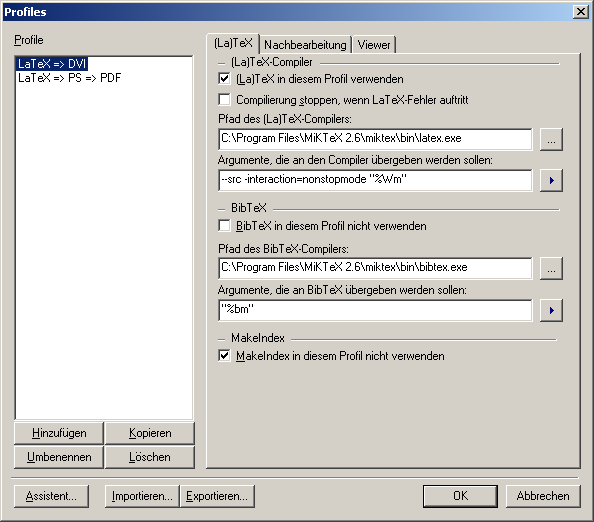
\includegraphics[width=0.49\textwidth]{techniccenter-profile-dvi-26} &
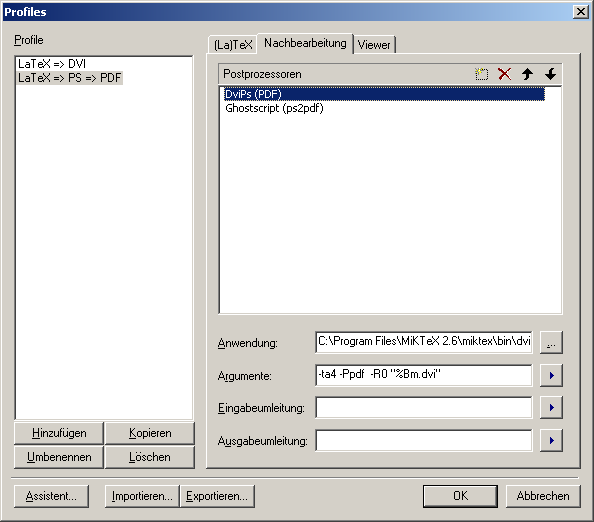
\includegraphics[width=0.49\textwidth]{techniccenter-profile-dvips-26} \\[4pt]
(a) & (b)
\end{tabular}
\caption{Spezifikation der Ausgabeprofile in TeXnicCenter.}
\label{fig:techniccenter-profile-latex}
\end{figure}

Für diese Vorlage wird die verwendung des Ausgabeprofiels \texttt{LaTeX => PDF} empfohlen.

%
%In der Datei \verb!tc_output_profiles_sumatra.tco! sind  folgende beiden "`maßgeschneiderten"' Ausgabeprofile für TexNicCenter angelegt (Import über \textsf{Build} $\rightarrow$ \textsf{Define Output Profiles ...}):
%\begin{itemize}
	%\item \verb!LaTeX => PDF (Sumatra)! -- Standard, direkte Erzeugung von PDF,
	%\item \verb!LaTeX => PS => PDF (Sumatra)! -- PDF "`klassisch"' via DVI und PS.
%\end{itemize}
%
%
%
%\subsubsection{Profil "`\texttt{LaTeX => PDF (Sumatra)}"'}
%
%Das ist das mit diesem Setup normalerweise verwendete Standardprofil.
%
%\paragraph{(La)Tex:}
%\begin{itemize}
  %\item Path to the (La)TeX compiler: \\
        %\begin{small} \verb!C:\Program Files\MiKTeX 2.8\miktex\bin\pdflatex.exe!\end{small}
  %\item Command line arguments to pass to the compiler:\\
%\begin{small}
   %\verb!-synctex=-1 -interaction=nonstopmode "%pm"!
%\end{small}
%\end{itemize}
%
%\paragraph{Postprocessor:} 
%leer, kein Postprocessor notwenig.
%
%\paragraph{Viewer:}
%\begin{itemize}
%\item Path of executable: \\
%\begin{small}
    %\verb!C:\Program Files\SumatraPDF\SumatraPDF.exe ! \\ 
    %\verb!-inverse-search "\"C:\Program Files\TeXnicCenter\TEXCNTR.EXE\" !\\
    %\verb!/ddecmd \"[goto('%f','%l')]\""!
%\end{small}
%%
%\item View project's output: \\
%\begin{small}
    %\checkbox\ Command line argument \\\
    %Command: \verb!"%bm.pdf"!
%\end{small}
%%
%\item Forward search:\\
%\begin{small}
    %\checkbox\ DDE command \\\
    %Command: \verb![ForwardSearch("%bm.pdf","%Wc",%l,0)]! \\
    %Server: \verb!SUMATRA! \\
    %Topic: \verb!Control!
%\end{small}
%\item Close document before running (La)TeX:\\
%\begin{small}
    %\checkbox\ Do not close
%\end{small}
%\end{itemize}
%
%
%
%
%\subsubsection{Profil "`\texttt{LaTeX => PS => PDF (Sumatra)}"'}
%
%Profil ausschließlich für den DVI-PS-Workflow (über DVI und PostScript).
%
%\paragraph{(La)Tex:}
%\begin{itemize}
  %\item Path to the (La)TeX compiler: \\
        %\begin{small} \verb!C:\Program Files\MiKTeX 2.8\miktex\bin\latex.exe!\end{small}
  %\item Command line arguments to pass to the compiler:\\
%\begin{small}
   %\verb!-synctex=-1 -interaction=nonstopmode "%pm"!
%\end{small}
%\end{itemize}
%
%\paragraph{Postprocessor:}
%\begin{itemize}
  %\item DviPS (PDF): \\
        %\begin{small} 
        %Executable: \verb!C:\Program Files\MiKTeX 2.8\miktex\bin\dvips.exe! \\
        %Arguments: \verb!-ta4 -P pdf -R0 "%Bm.dvi"!
        %\end{small}
  %\item Ghostscript (ps2pdf):\\
  		%\begin{small} 
        %Executable: \verb!C:\Program Files\gs\gs8.64\bin\gswin32c.exe! \\
        %Arguments: \verb!-q -dPDFSETTINGS=/prepress -sPAPERSIZE=a4 -dSAFER! \\
         %\verb!-dBATCH -dNOPAUSE -sDEVICE=pdfwrite -sOutputFile="%bm.pdf"! \\
         %\verb!-c save pop -f "%bm.ps"!
      %\end{small}
%\end{itemize}
%
%\paragraph{Viewer:}
%wie in Profil A. (\texttt{LaTeX => PDF (Sumatra)}).
	% Technische Ergänzungen
\chapter{Inhalt der CD-ROM/DVD}
\label{app:cdrom}

\paragraph{Format:} 
		CD-ROM, Single Layer, ISO9660-Format%
\footnote{Verwenden Sie möglichst ein Standardformat, bei DVDs natürlich
eine entsprechende andere Spezifikation.}


\section{PDF-Dateien}
\begin{FileList}{/}
\fitem{_Diplomarbeit.pdf} Diplomarbeit mit Instruktionen (Gesamtdokument)
%
\end{FileList}


\section{\latex-Dateien}

\textbf{Achtung:} Die folgende Auflistung soll nur den Gebrauch dieser Vorlage
erleichtern. Es ist bei einer Diplomarbeit \ia\ \emph{nicht} notwendig, die zugehörigen \latex-Dateien aufzulisten (wohl aber projektbezogene Dateien, Ergebnisse, Bilder, Kopien von Online-Literatur etc.)!
%\paragraph{Pfad:} \url{/}
\begin{FileList}{/}
\fitem{_Diplomarbeit.tex} Diplomarbeit (Hauptdokument) %
\fitem{vorwort.tex} Vorwort %
\fitem{kurzfassung.tex} Kurzfassung %
\fitem{abstract.tex} Abstract %
\fitem{einleitung.tex} Kapitel 1 %
\fitem{diplomschrift.tex} Kapitel 2 %
\fitem{latex.tex} Kapitel 3
\fitem{abbildungen.tex} Kapitel 4 %
\fitem{formeln.tex} Kapitel 5 %
\fitem{literatur.tex} Kapitel 6 %
\fitem{drucken.tex} Kapitel 7 %
\fitem{word.tex} Kapitel 8 %
\fitem{schluss.tex} Kapitel 9 %
\fitem{anhang_a.tex} Anhang A (Source Code) %
\fitem{anhang_b.tex} Anhang B (Inhalt CD-ROM) %
\fitem{anhang_c.tex} Anhang C (Änderungen) %
\fitem{anhang_d.tex} Anhang D (Latex Quellcode) %
\fitem{messbox.tex} Messbox zur Druckkontrolle %
\fitem{literatur.bib} Literatur-Datenbank (BibTeX-File)
\end{FileList}

\begin{comment}
\section{Dokumentation}
%\paragraph{Pfad:} \url{/docs/}
\begin{FileList}{/docs/}
\fitem{caption2.pdf}  \texttt{caption} Paket %
\fitem{fancyhdr.pdf} "`Fancy Headers"' Paket %
\fitem{float.pdf}     \texttt{float}
Paket \fitem{gerdoc.pdf}    Kurzbeschreibung zu \texttt{german.sty}
und \texttt{ngerman.sty} \fitem{grfguide.pdf}  \texttt{graphicx} Paket
\fitem{l2kurz.pdf}    \latex-Anleitung (deutsch)
\fitem{lshort.pdf}    \latex-Anleitung (englisch)
\fitem{subfigure.pdf} \texttt{subfigure} Paket
\fitem{symbols-a4.pdf} Verzeichnis aller \latex-Symbole
\end{FileList}
\end{comment}

\section{Style/Class-Dateien}
%\paragraph{Pfad:} \url{/}
\begin{FileList}{/}
\fitem{htldipl.sty} Class-File für dieses Dokument
\fitem{htl.sty} Style-File für dieses Dokument
\fitem{algorithmicx.sty}  \texttt{algorithmicx} Paket (Version 1.1) 
\fitem{algpseudocode.sty} \texttt{algpseudocode} Paket 
\fitem{listings2.cfg} \texttt{listings2} Paket 
\fitem{listings2.sty} \texttt{listings2} Paket 
\fitem{lstaspects.sty} \texttt{listings2} Paket 
\fitem{lstdoc2.sty} \texttt{listings2} Paket 
\fitem{lstlanguages.sty} \texttt{listings2} Paket 
\end{FileList}


\section{Sonstiges}
\begin{FileList}{/images}
\fitem{*.ai} Original Adobe Illustrator-Dateien %
\fitem{*.fh11} Original Macromedia Freehand-Dateien %
\fitem{*.jpg} Original Rasterbilder %
\fitem{*.eps} Bilder und Grafiken im EPS-Format%
%\fitem{fonts-bakoma/} BaKoMa TrueType Fonts %
\end{FileList}
	% Inhalt der CD-ROM/DVD
\chapter{Chronologische Liste der Änderungen}

\begin{sloppypar}
\begin{description}

\item[2010/11/22]
Überarbeitung der originalen Vorlagen von Dr.\ Wilhelm Burger und Anpassung an
die Bedürfnisse einer HTL-
Wichtigste Änderungen:
\begin{itemize}
  \item Wechsel auf UTF8
  \item Wechsel auf listings2-beta
  \item Neue Code-Umgebungen für Python und C\#
  \item Vorlagen für Normen und Patente im Literaturverzeichnis
  \item Hinweise auf DVI-PS Workflow entfernt
  \item Kapitel zur automatischen \latex-Code erzeugung hinzugefügt
\end{itemize}
%
\end{description}

\end{sloppypar}

%\section*{To Do} 
%\begin{itemize}
%\item Literaturempfehlungen zum Schreiben von Diplomarbeiten
%\item Hinweise für Literatursuche (Bibliotheksverbund, CiteSeer,...)
%\end{itemize}



	% Chronologische Liste der Änderungen
\chapter{\latex-Quellkode}
\label{app:latex}

\section*{Hauptdatei {\tt\_Diplomarbeit.tex}}

\begin{footnotesize}
\verbatiminput{_Diplomarbeit.tex}
\end{footnotesize}


%\vspace*{2cm}
\hrule
\hrule

\paragraph{Anmerkung:}
Das sollte nur ein \emph{Beispiel} für die Einbindung von Quellcode
in einem Anhang sein. Der \latex-Quellkode der eigenen
Diplomarbeit ist meist \emph{nicht} interessant genug, um ihn hier
wiederzugeben!

	% Quelltext dieses Dokuments

%%%----------------------------------------------------------
%Ausgabe der automatischen Zusatzdaten: Glossar, Index, Literaturverzeichnis
\clearpage
\printglossaries

\clearpage
\chapter*{Index}
\addcontentsline{toc}{chapter}{Index}
\printindex[allgemein]

\printindex

\printindex[name]

\printindex[title]


%Literaturverzeichnis
\clearpage
\addcontentsline{toc}{chapter}{\bibname}

\printbibliography


%%%----------------------------------------------------------

%%%Messbox zur Druckkontrolle
%\chapter*{Messbox zur Druckkontrolle}



\begin{center}
{\Large --- Druckgröße kontrollieren! ---}

\bigskip

\Messbox{100}{50} % Angabe der Breite/Hoehe in mm

\bigskip

{\Large --- Diese Seite nach dem Druck entfernen! ---}

\end{center}



\end{document}
